\documentclass[12pt,a4paper]{article}
\usepackage[utf8]{inputenc}
\usepackage[margin=1in]{geometry}
\usepackage{graphicx}
\usepackage{hyperref}
\usepackage{booktabs}
\usepackage{longtable}
\usepackage{enumitem}
\usepackage{tabularx}
\usepackage{float}
\usepackage{xcolor}
\usepackage{listings}
\usepackage{titlesec}
\usepackage{fancyhdr}
\usepackage{tocloft}
\usepackage{pdflscape}
\usepackage{needspace}
\usepackage{array}
\usepackage{adjustbox}
\usepackage[htt]{hyphenat}

% Allow slightly sloppy line breaking to prevent overfull hbox in description items
\tolerance=2000
\emergencystretch=2em

\hypersetup{
    colorlinks=true,
    linkcolor=blue,
    urlcolor=blue,
    citecolor=blue
}

\pagestyle{fancy}
\fancyhf{}
\fancyhead[L]{PageForge --- SRS \& Design Document}
\fancyhead[R]{Version 1.0}
\fancyfoot[C]{\thepage}

\title{
    \vspace{-1cm}
    \textbf{Software Requirements Specification}\\
    \textbf{and Design Document}\\[0.5cm]
    \Large{for}\\[0.5cm]
    \Huge{\textbf{PageForge}}\\[0.3cm]
    \Large{Self-Hosted Static Site Deployment Platform}\\[1cm]
    \large{Version 1.0 Approved}
}

\author{
    \textbf{Prepared by:} Praveen\\
    \textbf{Organization:} PageForge Project\\
    \textbf{Date:} February 24, 2026
}

\date{}

% Prevent orphaned headings (headings at bottom of page with no content following)
\raggedbottom
\widowpenalty=10000
\clubpenalty=10000

% Prevent headings from appearing at the bottom of a page with no content after them
% Using titlesec's \titlespacing with sufficient \needspace via before-code
\makeatletter
\renewcommand\section{\@startsection{section}{1}{\z@}%
  {-3.5ex \@plus -1ex \@minus -.2ex}%
  {2.3ex \@plus .2ex}%
  {\needspace{6\baselineskip}\normalfont\Large\bfseries}}
\renewcommand\subsection{\@startsection{subsection}{2}{\z@}%
  {-3.25ex\@plus -1ex \@minus -.2ex}%
  {1.5ex \@plus .2ex}%
  {\needspace{5\baselineskip}\normalfont\large\bfseries}}
\renewcommand\subsubsection{\@startsection{subsubsection}{3}{\z@}%
  {-3.25ex\@plus -1ex \@minus -.2ex}%
  {1.5ex \@plus .2ex}%
  {\needspace{4\baselineskip}\normalfont\normalsize\bfseries}}
\renewcommand\paragraph{\@startsection{paragraph}{4}{\z@}%
  {3.25ex \@plus 1ex \@minus .2ex}%
  {-1em}%
  {\needspace{4\baselineskip}\normalfont\normalsize\bfseries}}
\makeatother

\begin{document}

\maketitle
\thispagestyle{empty}
\newpage

% Revision History
\section*{Revision History}
\begin{tabularx}{\textwidth}{|l|l|X|l|}
\hline
\textbf{Name} & \textbf{Date} & \textbf{Reason For Changes} & \textbf{Version} \\
\hline
Praveen & 2026-02-24 & Initial SRS and Design document & 1.0 \\
\hline
\end{tabularx}
\newpage

\tableofcontents
\newpage

%===============================================================
% SECTION 1: INTRODUCTION
%===============================================================
\section{Introduction}

\subsection{Purpose}
This Software Requirements Specification (SRS) document describes the complete functional and non-functional requirements for \textbf{PageForge}, a self-hosted static site deployment platform, version 1.0. PageForge enables developers to build, deploy, and serve static websites from Git repositories or ZIP archives with automated build pipelines, custom domain support, and GitHub integration. This document covers the entire system including the web dashboard, REST API, build worker, and infrastructure components.

\subsection{Document Conventions}
\begin{itemize}
    \item \textbf{Bold text} is used for emphasis and key terms.
    \item \texttt{Monospace text} is used for code, file paths, API endpoints, and technical identifiers.
    \item Requirements are identified with unique tags: \texttt{FR-XX} for functional requirements, \texttt{NFR-XX} for non-functional requirements.
    \item Use cases are identified as \texttt{UC-XX}.
    \item Design artifacts are identified as \texttt{D-CL-XX} (class diagrams), \texttt{D-SQ-XX} (sequence diagrams), \texttt{D-DB-XX} (database), \texttt{D-SEC-XX} (security).
    \item Priority levels: \textbf{High} (essential for core functionality), \textbf{Medium} (important but not blocking), \textbf{Low} (nice-to-have).
    \item Higher-level requirement priorities are inherited by their child requirements unless explicitly overridden.
\end{itemize}

\subsection{Intended Audience and Reading Suggestions}
This document is intended for:
\begin{itemize}
    \item \textbf{Developers:} Sections 3--5 for system features, design, and architecture. Start with Section 4.1 (System Architecture) for an overview.
    \item \textbf{Project Managers:} Sections 1--2 for scope and overview, Section 5 for traceability.
    \item \textbf{Testers:} Sections 3.1--3.10 for feature requirements and stimulus/response sequences, Section 4.2 for sequence diagrams.
    \item \textbf{Evaluators:} Section 4 (Software Design) for architecture, class diagrams, sequence diagrams, database schema, and security design. Section 5 for requirement-to-design traceability.
    \item \textbf{End Users:} Sections 1.4, 2.1--2.3 for product scope and user classes.
\end{itemize}

\subsection{Product Scope}
PageForge is a self-hosted alternative to platforms like Vercel and Netlify, focused exclusively on static site deployment. It provides:
\begin{itemize}
    \item A web dashboard for managing projects, deployments, environment variables, and custom domains.
    \item Git-based deployment from GitHub repositories (public and private) with OAuth integration.
    \item ZIP file upload as an alternative deployment source.
    \item Dockerized build pipelines with configurable build commands, resource limits, and security isolation.
    \item Automatic static site serving via Caddy reverse proxy with dynamic route management.
    \item S3-compatible artifact storage via MinIO.
    \item Multi-user authentication with email/password credentials, OTP-based email verification during registration, and OTP-based password reset.
    \item Real-time build log streaming via WebSocket and Redis Pub/Sub.
\end{itemize}

The platform is designed for individual developers or small teams who want full control over their deployment infrastructure without vendor lock-in.

\subsection{References}
\begin{enumerate}
    \item Next.js 14 Documentation: \url{https://nextjs.org/docs}
    \item NextAuth.js v5 (Auth.js) Documentation: \url{https://authjs.dev}
    \item MongoDB/Mongoose Documentation: \url{https://mongoosejs.com/docs/}
    \item BullMQ Documentation: \url{https://docs.bullmq.io/}
    \item Docker Engine API: \url{https://docs.docker.com/engine/api/}
    \item Caddy Server Admin API: \url{https://caddyserver.com/docs/api}
    \item MinIO JavaScript Client: \href{https://min.io/docs/minio/linux/developers/javascript/minio-javascript.html}{\texttt{min.io/docs/.../minio\allowbreak{}-javascript.html}}
    \item GitHub OAuth Documentation:\newline \url{https://docs.github.com/en/apps/oauth-apps}
    \item Roger S. Pressman, \textit{Software Engineering: A Practitioner's Approach}, Appendix A.
    \item IEEE Std 830-1998, \textit{IEEE Recommended Practice for Software Requirements Specifications}.
\end{enumerate}

\newpage

%===============================================================
% SECTION 2: OVERALL DESCRIPTION
%===============================================================
\section{Overall Description}

\subsection{Product Perspective}
PageForge is a new, self-contained product that fills the gap between fully managed deployment platforms (Vercel, Netlify) and manual server configuration. It is designed to run entirely on a user's own infrastructure --- a single Linux server with Docker --- eliminating dependency on third-party hosting services.

The system consists of four major subsystems:
\begin{enumerate}
    \item \textbf{Web Application (Next.js 14):} Dashboard UI and REST API server.
    \item \textbf{Build Worker:} Background job processor that executes builds in Docker containers.
    \item \textbf{Infrastructure Services:} MongoDB, Redis, MinIO, and Caddy running as Docker containers.
    \item \textbf{External Integrations:} GitHub OAuth and GitHub API for repository access.
\end{enumerate}

\begin{figure}[H]
    \centering
    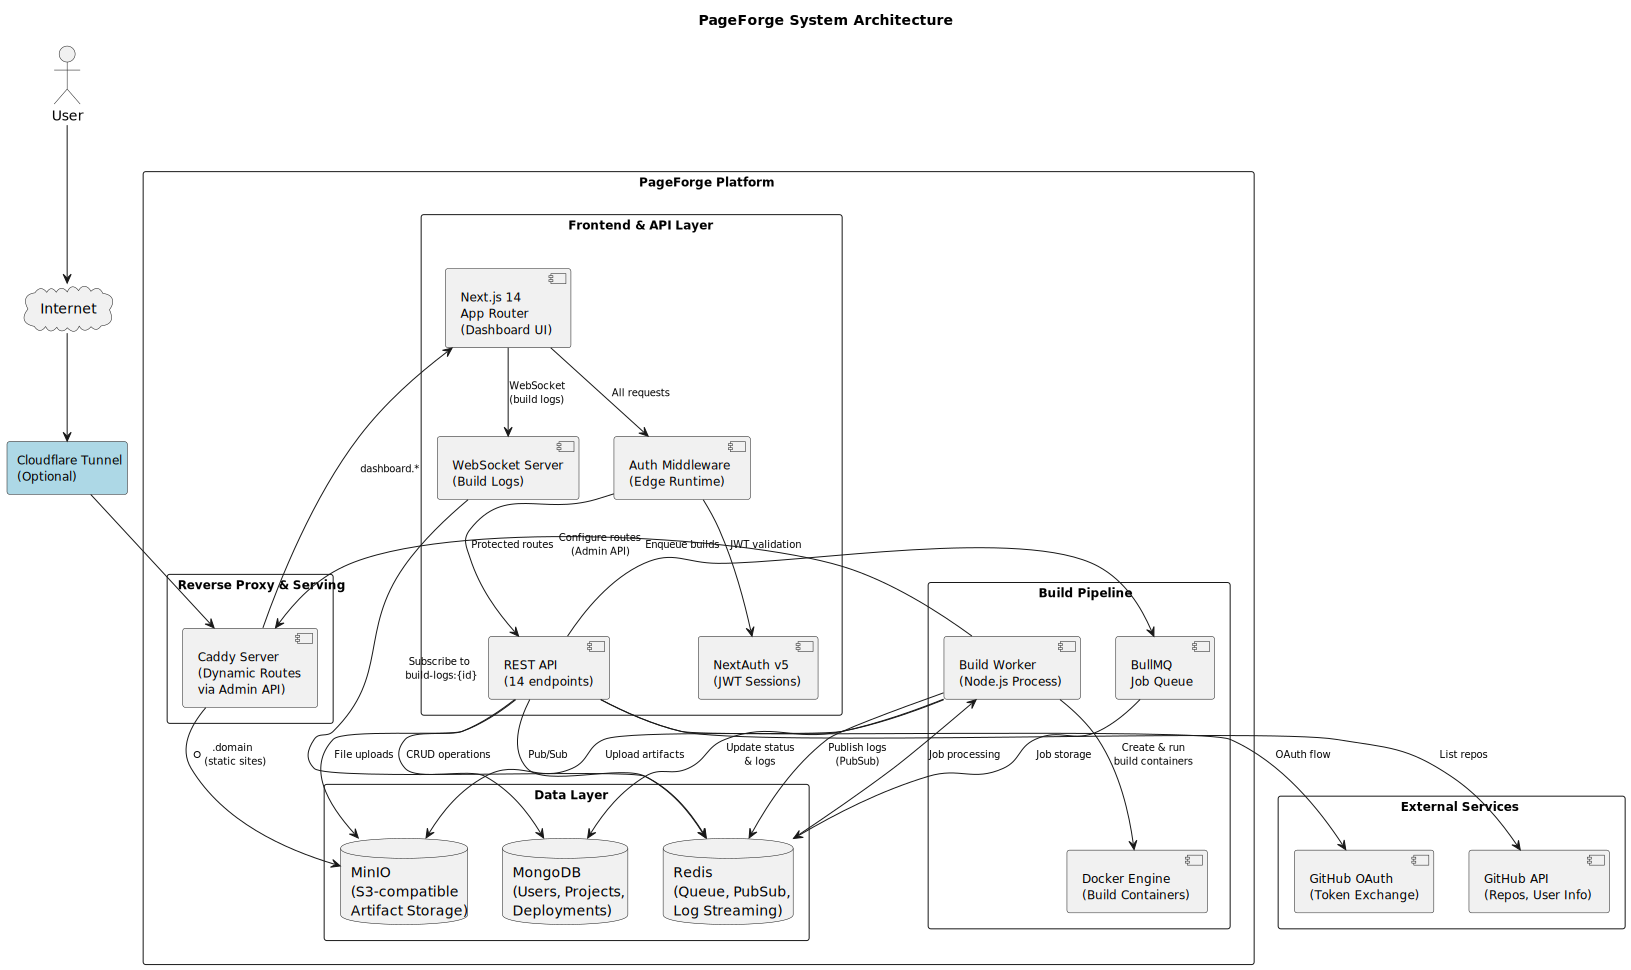
\includegraphics[width=\textwidth]{diagrams/architecture.pdf}
    \caption{PageForge System Architecture Overview}
    \label{fig:architecture}
\end{figure}

\subsection{Product Functions}
The major functions of PageForge are:
\begin{itemize}
    \item \textbf{User Authentication:} Registration with email OTP verification, login (email/password), forgot password via OTP, session management, logout.
    \item \textbf{GitHub OAuth Integration:} Connect/disconnect GitHub account, import private repositories.
    \item \textbf{Project Management:} Create, read, update, delete projects with Git or ZIP sources.
    \item \textbf{Deployment Pipeline:} Trigger builds, execute in Docker containers, stream logs, store artifacts.
    \item \textbf{Environment Variables:} Configure build-time environment variables per project.
    \item \textbf{Custom Domains:} Add custom domains, verify via DNS CNAME, configure routing.
    \item \textbf{Static Site Serving:} Serve deployed sites via Caddy with automatic subdomain routing.
    \item \textbf{Build Log Viewer:} Real-time streaming of build output with stdout/stderr separation.
\end{itemize}

\subsection{User Classes and Characteristics}
\begin{enumerate}
    \item \textbf{Developer (Primary User):} Technical users who deploy static websites. They interact with all features: project creation, deployment, domain management, and GitHub integration. Expected to understand Git, build tools (npm/yarn), and DNS configuration.
    \item \textbf{Administrator:} The person who installs and maintains the PageForge server. Responsible for Docker, DNS, and infrastructure configuration. May also be a developer user.
    \item \textbf{End Visitor:} Visitors who access the deployed static sites. They interact only with the served content through Caddy, not with the PageForge dashboard.
\end{enumerate}

\subsection{Operating Environment}
\begin{itemize}
    \item \textbf{Server OS:} Linux (tested on Arch Linux; compatible with any Linux distribution with Docker).
    \item \textbf{Runtime:} Node.js 20+ (LTS), Docker Engine 24+.
    \item \textbf{Database:} MongoDB 7.0+.
    \item \textbf{Cache/Queue:} Redis 7.0+.
    \item \textbf{Object Storage:} MinIO (S3-compatible).
    \item \textbf{Reverse Proxy:} Caddy 2.x with JSON admin API.
    \item \textbf{Package Manager:} pnpm 8+ with workspace support.
    \item \textbf{Browser:} Modern browsers (Chrome 90+, Firefox 90+, Safari 15+, Edge 90+).
    \item \textbf{Optional:} Cloudflare Tunnel for public access without port forwarding.
\end{itemize}

\subsection{Design and Implementation Constraints}
\begin{itemize}
    \item \textbf{Monorepo Structure:} pnpm workspace with three packages (\texttt{apps/web}, \texttt{apps/worker}, \texttt{packages/shared}).
    \item \textbf{TypeScript Only:} All code must be written in TypeScript with strict type checking.
    \item \textbf{Edge Runtime Compatibility:} Middleware must not import Node.js-only modules (Mongoose, bcrypt) due to Next.js Edge Runtime restrictions.
    \item \textbf{Docker Dependency:} Build execution requires Docker Engine access via socket (\texttt{/var/run/docker.sock}).
    \item \textbf{Static Sites Only:} Only static site output (HTML/CSS/JS) is supported; no server-side rendering or serverless functions in deployed sites.
    \item \textbf{GitHub OAuth Scope:} The \texttt{repo} scope grants read and write access; GitHub does not offer a read-only scope for private repositories via OAuth Apps.
\end{itemize}

\subsection{User Documentation}
\begin{itemize}
    \item \texttt{README.md} --- Installation and quick start guide.
    \item \texttt{.env.example} --- Environment variable reference with descriptions.
    \item In-app contextual help text on forms and configuration screens.
\end{itemize}

\subsection{Assumptions and Dependencies}
\begin{itemize}
    \item Docker Engine is installed and accessible via the Docker socket.
    \item MongoDB, Redis, and MinIO are running (provided via \texttt{docker-compose.yml}).
    \item The server has internet access for cloning Git repositories and pulling Docker images.
    \item DNS for the base domain (\texttt{*.itspraveen.dpdns.org}) is configured with wildcard resolution pointing to the server.
    \item For GitHub OAuth: a GitHub OAuth App is created with correct client ID, secret, and callback URL.
    \item The \texttt{node:20-alpine} Docker image is available (pulled automatically on first build).
    \item For custom domains: users can configure CNAME records on their DNS provider.
\end{itemize}

\newpage

%===============================================================
% SECTION 3: SYSTEM FEATURES (FUNCTIONAL REQUIREMENTS)
%===============================================================
\section{System Features}

\subsection{User Registration}
\subsubsection{Description and Priority}
Allows new users to create an account with name, email, and password. Email address is verified via OTP before account creation (see Section 3.3). \textbf{Priority: High.}

\subsubsection{Stimulus/Response Sequences}
\begin{enumerate}
    \item User navigates to \texttt{/register}.
    \item User enters name, email, and password.
    \item System validates input and checks email uniqueness.
    \item System sends a 6-digit OTP to the provided email.
    \item User enters the OTP on the verification screen.
    \item System verifies OTP and creates user account with hashed password.
    \item System redirects to login page.
\end{enumerate}

\subsubsection{Functional Requirements}
\begin{description}
    \item[FR-01] The system shall provide a registration form accepting name, email, and password.
    \item[FR-02] The system shall validate that all fields are non-empty and email is in valid format.
    \item[FR-03] The system shall reject registration if the email is already registered (HTTP 409).
    \item[FR-04] The system shall hash passwords using bcrypt with 12 salt rounds before storage.
    \item[FR-05] The system shall require email OTP verification before finalizing account creation (see Section 3.3).
    \item[FR-06] The system shall store the user in MongoDB with \texttt{createdAt} and \texttt{updatedAt} timestamps only after successful OTP verification, and return HTTP 201.
    \item[FR-07] The system shall redirect authenticated users away from the registration page to the dashboard.
\end{description}

\subsection{User Login (Credentials)}
\subsubsection{Description and Priority}
Allows registered users to authenticate with email and password. \textbf{Priority: High.}

\subsubsection{Stimulus/Response Sequences}
\begin{enumerate}
    \item User navigates to \texttt{/login}.
    \item User enters email and password.
    \item System verifies credentials against stored hash.
    \item System issues JWT session token (30-day expiry).
    \item System redirects to dashboard.
\end{enumerate}

\subsubsection{Functional Requirements}
\begin{description}
    \item[FR-08] The system shall provide a login form accepting email and password.
    \item[FR-09] The system shall authenticate users via NextAuth.js Credentials provider.
    \item[FR-10] The system shall compare submitted password against stored bcrypt hash.
    \item[FR-11] The system shall issue a JWT token containing user ID, name, and email upon successful authentication.
    \item[FR-12] The system shall set the JWT session cookie with a maximum age of 30 days.
    \item[FR-13] The system shall display ``Invalid email or password'' for failed authentication (without revealing which field is incorrect).
    \item[FR-14] The system shall redirect authenticated users away from the login page.
\end{description}

\subsection{Email OTP Verification (Registration)}
\subsubsection{Description and Priority}
Verifies a user's email address during registration by sending a one-time password (OTP) to the provided email. The user must enter the correct OTP to complete account creation. This ensures only valid, accessible email addresses are registered. \textbf{Priority: High.}

\subsubsection{Stimulus/Response Sequences}
\begin{enumerate}
    \item User fills in the registration form (name, email, password) and submits.
    \item System validates input and checks email uniqueness.
    \item System generates a 6-digit OTP and sends it to the provided email.
    \item User enters the OTP on the verification screen.
    \item System verifies the OTP.
    \item On success, the system creates the user account and redirects to login.
\end{enumerate}

\subsubsection{Functional Requirements}
\begin{description}
    \item[FR-15] The system shall send a 6-digit OTP to the user's email after initial registration form submission, before creating the account.
    \item[FR-16] The system shall generate a cryptographically random 6-digit OTP.
    \item[FR-17] The system shall store the pending registration data and OTP temporarily until verification completes or expires.
    \item[FR-18] The system shall expire OTPs after 5 minutes.
    \item[FR-19] The system shall invalidate an OTP after successful verification (single-use).
    \item[FR-20] The system shall reject expired or invalid OTPs with an appropriate error message.
    \item[FR-21] The system shall create the user account only after successful OTP verification.
    \item[FR-22] The system shall allow the user to request a new OTP if the previous one expired.
\end{description}

\subsection{GitHub OAuth Connection}
\subsubsection{Description and Priority}
Allows users to connect their GitHub account for importing private repositories. \textbf{Priority: High.}

\subsubsection{Stimulus/Response Sequences}
\begin{enumerate}
    \item User navigates to \texttt{/settings} and clicks ``Connect GitHub''.
    \item System redirects to GitHub OAuth authorization page.
    \item User authorizes PageForge with \texttt{repo} scope.
    \item GitHub redirects back with authorization code.
    \item System exchanges code for access token and stores it.
    \item User is redirected to settings with success status.
\end{enumerate}

\subsubsection{Functional Requirements}
\begin{description}
    \item[FR-23] The system shall redirect to GitHub OAuth with \texttt{client\_id}, \texttt{redirect\_uri}, \texttt{scope=repo}, and \texttt{state=userId}.
    \item[FR-24] The system shall exchange the authorization code for an access token via GitHub's token endpoint.
    \item[FR-25] The system shall fetch the GitHub user profile (ID, username) using the access token.
    \item[FR-26] The system shall store the access token, GitHub ID, username, and connection timestamp on the User document.
    \item[FR-27] The system shall store the GitHub access token with \texttt{select: false} (never exposed in API responses).
    \item[FR-28] The system shall provide a ``Disconnect GitHub'' action that removes all GitHub fields from the User.
    \item[FR-29] The system shall provide a status endpoint returning connection state, username, and connection date.
    \item[FR-30] The system shall handle OAuth errors (user denial, invalid code) gracefully with redirect to settings page with error parameter.
\end{description}

\subsection{Project Management}
\subsubsection{Description and Priority}
Allows users to create, view, update, and delete static site projects. \textbf{Priority: High.}

\subsubsection{Stimulus/Response Sequences}
\begin{enumerate}
    \item User creates a project via the 3-step wizard (name, source, build config).
    \item System generates a unique slug and stores the project.
    \item User can view project list on the dashboard.
    \item User can update project settings (name, source, build commands).
    \item User can delete a project.
\end{enumerate}

\subsubsection{Functional Requirements}
\begin{description}
    \item[FR-31] The system shall provide a 3-step project creation wizard: (1) Name \& Source Type, (2) Source Configuration, (3) Build Configuration.
    \item[FR-32] The system shall auto-generate a URL-safe slug from the project name.
    \item[FR-33] The system shall support two source types: \texttt{git} and \texttt{zip}.
    \item[FR-34] For Git sources, the system shall accept repository URL, branch, and provider (GitHub or Other).
    \item[FR-35] When GitHub is connected, the system shall display a searchable repository picker populated from the GitHub API.
    \item[FR-36] The system shall store default build configuration: \texttt{installCommand} (``npm install''), \texttt{buildCommand} (``npm run build''), \texttt{outputDirectory} (``dist'').
    \item[FR-37] The system shall scope all projects to the authenticated user via \texttt{userId}.
    \item[FR-38] The system shall enforce unique slugs across all projects.
    \item[FR-39] The system shall support updating project name, source config, and build config via PATCH.
    \item[FR-40] The system shall support deleting a project via DELETE.
    \item[FR-41] The system shall list only projects belonging to the authenticated user.
    \item[FR-42] The system shall accept an optional Personal Access Token (PAT) per project for Git authentication.
    \item[FR-43] The system shall support removing a project-level PAT via \texttt{removeGitToken} flag.
\end{description}

\subsection{Deployment Pipeline}
\subsubsection{Description and Priority}
Executes builds in isolated Docker containers and serves the resulting static assets. \textbf{Priority: High.}

\subsubsection{Stimulus/Response Sequences}
\begin{enumerate}
    \item User clicks ``Deploy'' on a project.
    \item System creates a deployment record (status: \texttt{queued}).
    \item System enqueues a build job via BullMQ/Redis.
    \item Worker picks up the job, creates a Docker container, and executes the build.
    \item Worker streams build logs to Redis Pub/Sub and MongoDB.
    \item On success, worker uploads artifacts to MinIO and configures Caddy route.
    \item Deployment status updates to \texttt{ready} or \texttt{failed}.
\end{enumerate}

\subsubsection{Functional Requirements}
\begin{description}
    \item[FR-44] The system shall create a deployment record with status \texttt{queued} and a source snapshot.
    \item[FR-45] The system shall resolve Git authentication tokens in priority order: project PAT > user GitHub OAuth token > none (public repos).
    \item[FR-46] The system shall enqueue the build job to BullMQ via Redis.
    \item[FR-47] The worker shall create a Docker container using the \texttt{node:20-alpine} image.
    \item[FR-48] The worker shall configure container resource limits: memory (512MB default), CPU (1 core default).
    \item[FR-49] The worker shall set \texttt{no-new-privileges} security option on containers.
    \item[FR-50] The worker shall optionally use gVisor runtime (\texttt{runsc}) when \texttt{GVISOR\_ENABLED=true}.
    \item[FR-51] The worker shall inject environment variables from the project configuration into the container.
    \item[FR-52] The worker shall inject \texttt{GIT\_AUTH\_TOKEN} as an environment variable and configure Git credential helper.
    \item[FR-53] The worker shall automatically install \texttt{git} in the container if not present.
    \item[FR-54] The worker shall clone the Git repository (or extract ZIP) and execute build commands.
    \item[FR-55] The worker shall parse Docker multiplexed stream format (8-byte header) for stdout/stderr separation.
    \item[FR-56] The worker shall sanitize all secrets from build log output.
    \item[FR-57] The worker shall publish log entries to Redis Pub/Sub channel \texttt{build\allowbreak{}-logs:\allowbreak{}\{deploymentId\}}.
    \item[FR-58] The worker shall persist log entries to the deployment's \texttt{buildLogs} array in MongoDB.
    \item[FR-59] The worker shall extract the build output directory as a tar archive from the container.
    \item[FR-60] The worker shall upload the extracted build artifacts to MinIO under the path \texttt{artifacts/\allowbreak{}\{deploymentId\}/}.
    \item[FR-61] The worker shall configure a Caddy route mapping \texttt{\{slug\}.\allowbreak{}\{domain\}} to the MinIO artifact path.
    \item[FR-62] The worker shall update deployment status through the lifecycle: \texttt{queued} $\rightarrow$ \texttt{building} $\rightarrow$ \texttt{uploading} $\rightarrow$ \texttt{ready} (or \texttt{failed}).
    \item[FR-63] The worker shall remove the Docker container after build completion (success or failure).
    \item[FR-64] The system shall list deployments for a project sorted by creation date (newest first).
    \item[FR-65] The system shall provide a deployment detail view with build logs and status.
\end{description}

\subsection{Environment Variables}
\subsubsection{Description and Priority}
Allows users to configure build-time environment variables per project. \textbf{Priority: Medium.}

\subsubsection{Stimulus/Response Sequences}
\begin{enumerate}
    \item User navigates to the Environment tab on a project page.
    \item User adds, edits, or removes key-value pairs.
    \item User saves changes.
    \item Variables are injected into Docker containers during deployment.
\end{enumerate}

\subsubsection{Functional Requirements}
\begin{description}
    \item[FR-66] The system shall store environment variables as an array of \texttt{\{key, value, encrypted\}} objects on the Project document.
    \item[FR-67] The system shall provide GET and PUT endpoints for environment variables at \texttt{/api/projects/\{slug\}/env}.
    \item[FR-68] The system shall replace all environment variables atomically on PUT (full replacement, not merge).
    \item[FR-69] The system shall inject all project environment variables into the Docker build container.
    \item[FR-70] The system shall mask environment variable values in the UI.
\end{description}

\subsection{Custom Domain Management}
\subsubsection{Description and Priority}
Allows users to map custom domains to their deployed projects. \textbf{Priority: Medium.}

\subsubsection{Stimulus/Response Sequences}
\begin{enumerate}
    \item User adds a custom domain on the Domains tab.
    \item System provides a CNAME target for DNS configuration.
    \item User configures CNAME record at their DNS provider.
    \item User clicks ``Verify'' to trigger DNS verification.
    \item System verifies CNAME and configures Caddy route for the custom domain.
\end{enumerate}

\subsubsection{Functional Requirements}
\begin{description}
    \item[FR-71] The system shall accept custom domain input and validate format.
    \item[FR-72] The system shall generate a CNAME target of \texttt{\{slug\}.\{PAGEFORGE\_DOMAIN\}}.
    \item[FR-73] The system shall store domains as embedded documents with \texttt{domain}, \texttt{cnameTarget}, \texttt{verified}, and \texttt{verifiedAt} fields.
    \item[FR-74] The system shall verify custom domains by resolving CNAME records via DNS and comparing to the expected target.
    \item[FR-75] The system shall configure a Caddy route for verified custom domains pointing to the project's artifacts.
    \item[FR-76] The system shall support removing custom domains, including cleanup of Caddy routes.
    \item[FR-77] The system shall display domain verification status (Pending/Verified) in the UI.
\end{description}

\subsection{ZIP File Upload}
\subsubsection{Description and Priority}
Allows users to upload pre-built static site archives as an alternative to Git-based deployment. \textbf{Priority: Medium.}

\subsubsection{Stimulus/Response Sequences}
\begin{enumerate}
    \item User selects ``ZIP Upload'' as the source type during project creation.
    \item User uploads a ZIP file via the project page.
    \item System stores the file in MinIO.
    \item User triggers a deployment which uses the uploaded ZIP.
\end{enumerate}

\subsubsection{Functional Requirements}
\begin{description}
    \item[FR-78] The system shall accept ZIP file uploads via multipart form data at \texttt{/api/upload/\{slug\}}.
    \item[FR-79] The system shall store uploaded files in MinIO at \texttt{uploads/\{slug\}/\{filename\}}.
    \item[FR-80] The system shall update the project's \texttt{zipFileName} field after successful upload.
    \item[FR-81] The system shall use the uploaded ZIP as the source for deployment builds.
\end{description}

\subsection{Build Log Viewer}
\subsubsection{Description and Priority}
Provides real-time build log streaming during deployments. \textbf{Priority: Medium.}

\subsubsection{Stimulus/Response Sequences}
\begin{enumerate}
    \item User navigates to a deployment detail page.
    \item System establishes WebSocket connection to\\ \texttt{ws://\allowbreak{}\{host\}/\allowbreak{}ws/\allowbreak{}logs/\allowbreak{}\{deploymentId\}}.
    \item Build logs are streamed in real-time from Redis Pub/Sub.
    \item After build completes, historical logs are available from MongoDB.
\end{enumerate}

\subsubsection{Functional Requirements}
\begin{description}
    \item[FR-82] The system shall provide a WebSocket endpoint at \texttt{/ws/logs/\{deploymentId\}} for live log streaming.
    \item[FR-83] The WebSocket server shall subscribe to Redis Pub/Sub channel \texttt{build-logs:\{deploymentId\}}.
    \item[FR-84] The system shall forward log messages (type, stream, line, timestamp) to connected WebSocket clients.
    \item[FR-85] The system shall also poll the deployment API every 2 seconds as a fallback for log updates.
    \item[FR-86] The system shall display logs with visual distinction between stdout, stderr, and system messages.
    \item[FR-87] The system shall auto-scroll to the latest log entry.
    \item[FR-88] The system shall display deployment status (queued, building, uploading, ready, failed) with colored badges.
\end{description}

\subsection{Forgot Password (OTP-Based Password Reset)}
\subsubsection{Description and Priority}
Allows users to reset their password by verifying their identity via a one-time password sent to their registered email address. \textbf{Priority: High.}

\subsubsection{Stimulus/Response Sequences}
\begin{enumerate}
    \item User clicks ``Forgot Password'' on the login page.
    \item User enters their registered email address.
    \item System sends a 6-digit OTP to the email.
    \item User enters the OTP on the verification screen.
    \item System verifies the OTP and presents the password reset form.
    \item User enters and confirms a new password.
    \item System hashes the new password and updates the user record.
    \item System redirects to the login page with a success message.
\end{enumerate}

\subsubsection{Functional Requirements}
\begin{description}
    \item[FR-89] The system shall provide a ``Forgot Password'' link on the login page navigating to \texttt{/forgot-password}.
    \item[FR-90] The system shall accept an email address and send a 6-digit OTP to it if the email is registered.
    \item[FR-91] The system shall not reveal whether an email is registered or not (to prevent user enumeration).
    \item[FR-92] The system shall generate a cryptographically random 6-digit OTP with a 5-minute expiry.
    \item[FR-93] The system shall invalidate the OTP after successful verification (single-use).
    \item[FR-94] The system shall present a new password form only after successful OTP verification.
    \item[FR-95] The system shall validate that the new password meets minimum requirements.
    \item[FR-96] The system shall hash the new password using bcrypt with 12 salt rounds and update the user record.
    \item[FR-97] The system shall invalidate all existing sessions for the user after a password reset.
    \item[FR-98] The system shall redirect to the login page after successful password reset.
\end{description}

\newpage

%===============================================================
% SECTION 4: SOFTWARE DESIGN
%===============================================================
\section{Software Design}

\subsection{System Architecture}
PageForge follows a \textbf{modular monorepo architecture} with clear separation between the web application, build worker, and shared types. The system uses an \textbf{event-driven build pipeline} with BullMQ for job queuing and Redis Pub/Sub for real-time log streaming.

\subsubsection{Architecture Overview}
The system is divided into the following layers:

\begin{enumerate}
    \item \textbf{Presentation Layer:} Next.js 14 App Router with React components, TailwindCSS styling, and client-side hooks (\texttt{useFetch}, \texttt{useMutation}).
    \item \textbf{API Layer:} RESTful API with 14 route handlers, JWT authentication middleware, and ownership-scoped data access.
    \item \textbf{Business Logic Layer:} Auth config, GitHub OAuth flow, project/deployment management, build queue management.
    \item \textbf{Worker Layer:} BullMQ worker process, Docker executor, artifact manager, build logger.
    \item \textbf{Data Layer:} MongoDB (Mongoose ODM), Redis (queue + pub/sub), MinIO (S3 artifact storage).
    \item \textbf{Infrastructure Layer:} Caddy (reverse proxy + static serving), Docker Engine (build isolation), Cloudflare Tunnel (optional public access).
\end{enumerate}

\begin{figure}[H]
    \centering
    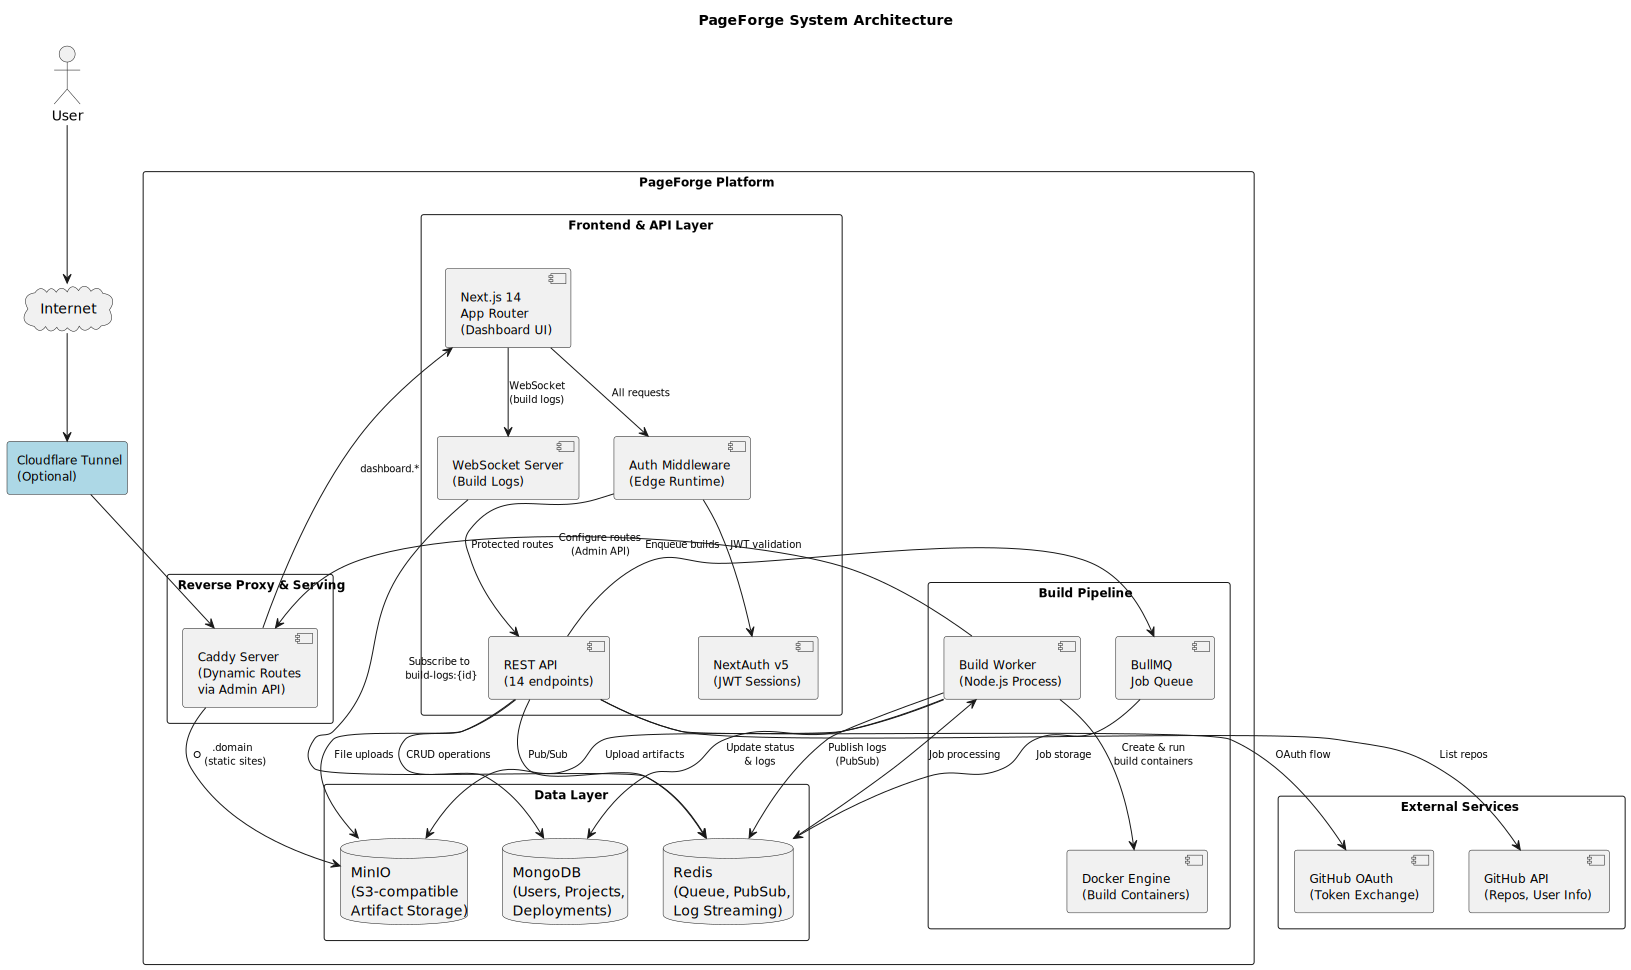
\includegraphics[width=\textwidth]{diagrams/architecture.pdf}
    \caption{System Architecture Diagram}
    \label{fig:arch}
\end{figure}

\subsubsection{Monorepo Structure}
\begin{verbatim}
PageForge/
  apps/
    web/          # Next.js 14 dashboard + API (Port 3000)
    worker/       # BullMQ build worker (background process)
  packages/
    shared/       # Shared TypeScript types and constants
  infra/
    docker-compose.yml  # MongoDB, Redis, MinIO, Caddy
    caddy.json          # Caddy server configuration
    init-minio.sh       # MinIO bucket initialization
\end{verbatim}

\subsubsection{API Endpoints}
{\footnotesize
\begin{longtable}{|l|>{\ttfamily\raggedright\arraybackslash}p{6cm}|>{\raggedright\arraybackslash}p{3.5cm}|}
\hline
\textbf{Method} & \textbf{\textrm{Endpoint}} & \textbf{Description} \\
\hline
\endfirsthead
\hline
\textbf{Method} & \textbf{\textrm{Endpoint}} & \textbf{Description} \\
\hline
\endhead
POST & /api/auth/register & User registration \\
\hline
GET/POST & /api/auth/[...nextauth] & NextAuth.js session management \\
\hline
POST & /api/auth/otp/send & Send OTP (registration or password reset) \\
\hline
POST & /api/auth/otp/verify & Verify OTP code \\
\hline
POST & /api/auth/forgot-password & Reset password after OTP verification \\
\hline
GET & /api/auth/github & Initiate GitHub OAuth flow \\
\hline
DELETE & /api/auth/github & Disconnect GitHub account \\
\hline
GET & /api/auth/github/callback & GitHub OAuth callback handler \\
\hline
GET & /api/auth/github/status & GitHub connection status \\
\hline
GET & /api/github/repos & List GitHub repositories \\
\hline
GET/POST & /api/projects & List / create projects \\
\hline
GET/PATCH/DELETE & /api/projects/[slug] & Get / update / delete project \\
\hline
GET/POST & /api/projects/[slug]/deployments & List / trigger deployments \\
\hline
GET & /api/projects/[slug]/\allowbreak{}deployments/[id] & Get deployment details \\
\hline
GET/PUT & /api/projects/[slug]/env & Get / set environment variables \\
\hline
GET/POST & /api/projects/[slug]/domains & List / add domains \\
\hline
POST/DELETE & /api/projects/[slug]/\allowbreak{}domains/[domain] & Verify / remove domain \\
\hline
POST & /api/upload/[slug] & Upload ZIP file \\
\hline
\end{longtable}
}

\subsection{Detailed Design}

\subsubsection{Class Diagrams}
The class diagram shows all major classes across the six modules: Authentication, Project Management, Deployment, Build Worker, Infrastructure, and GitHub Integration.

\begin{landscape}
\begin{figure}[p]
    \centering
    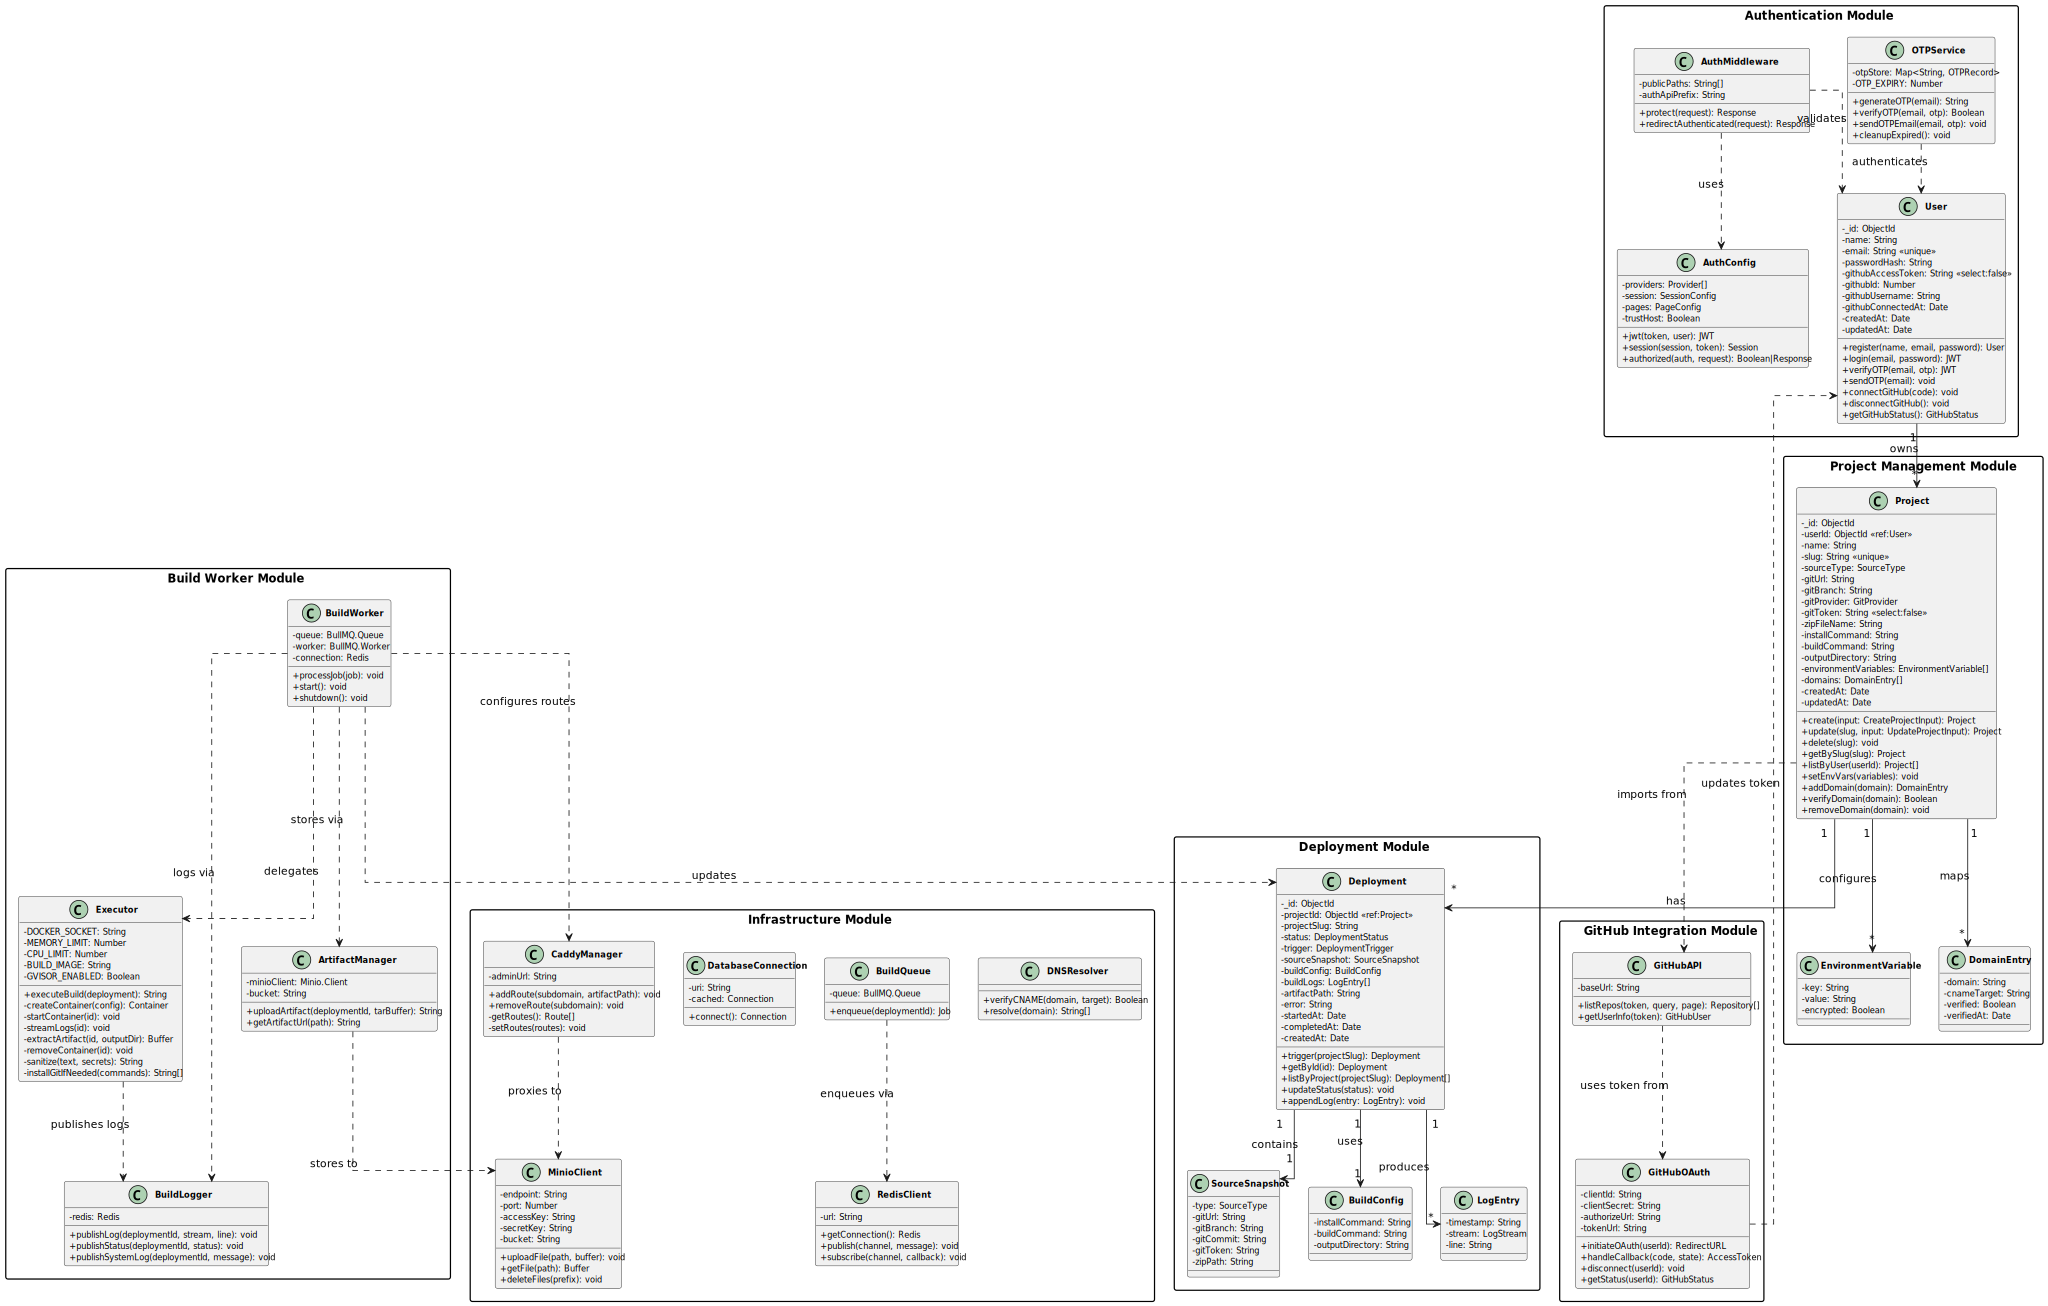
\includegraphics[width=\linewidth,height=0.85\textheight,keepaspectratio]{diagrams/class_diagram.pdf}
    \caption{Complete Class Diagram (D-CL-01)}
    \label{fig:class}
\end{figure}
\end{landscape}

\textbf{Key Design Decisions:}
\begin{itemize}
    \item \textbf{User} class owns Projects (1-to-many), and Projects own Deployments (1-to-many).
    \item \textbf{EnvironmentVariable}, \textbf{DomainEntry}, \textbf{SourceSnapshot}, \textbf{BuildConfig}, and \textbf{LogEntry} are embedded documents (not separate collections) for performance and atomicity.
    \item \textbf{Sensitive fields} (\texttt{passwordHash}, \texttt{githubAccessToken}, \texttt{gitToken}) use Mongoose \texttt{select: false} and are stripped in \texttt{toJSON}/\texttt{toObject} transforms.
    \item \textbf{BuildWorker} delegates to \textbf{Executor} (Docker), \textbf{ArtifactManager} (MinIO), and \textbf{BuildLogger} (Redis) following the single-responsibility principle.
    \item \textbf{OTPService} manages OTP generation, verification, and email delivery for registration email verification and password reset.
\end{itemize}

\subsubsection{Sequence Diagrams}

\paragraph{SD-01: User Registration}
\begin{figure}[H]
    \centering
    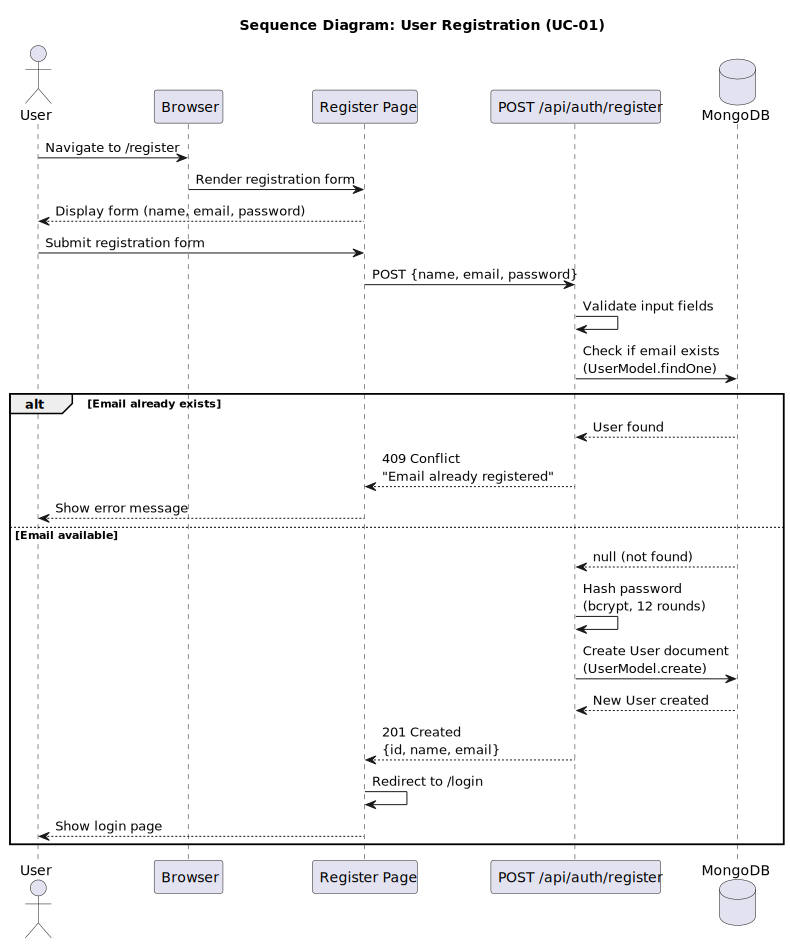
\includegraphics[width=0.9\textwidth]{diagrams/seq_register.pdf}
    \caption{Sequence Diagram: User Registration (D-SQ-01)}
    \label{fig:seq_register}
\end{figure}

\paragraph{SD-02: User Login (Credentials)}
\begin{figure}[H]
    \centering
    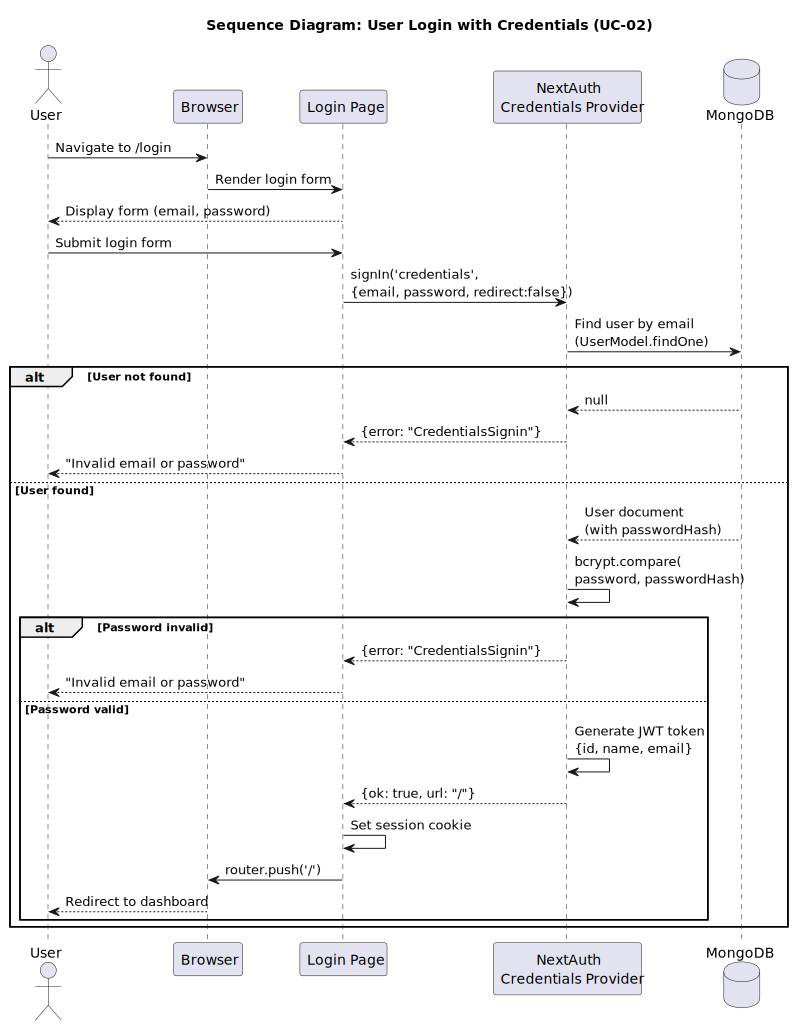
\includegraphics[width=0.9\textwidth]{diagrams/seq_login.pdf}
    \caption{Sequence Diagram: User Login with Credentials (D-SQ-02)}
    \label{fig:seq_login}
\end{figure}

\paragraph{SD-03: Email OTP Verification (Registration \& Password Reset)}
\begin{figure}[H]
    \centering
    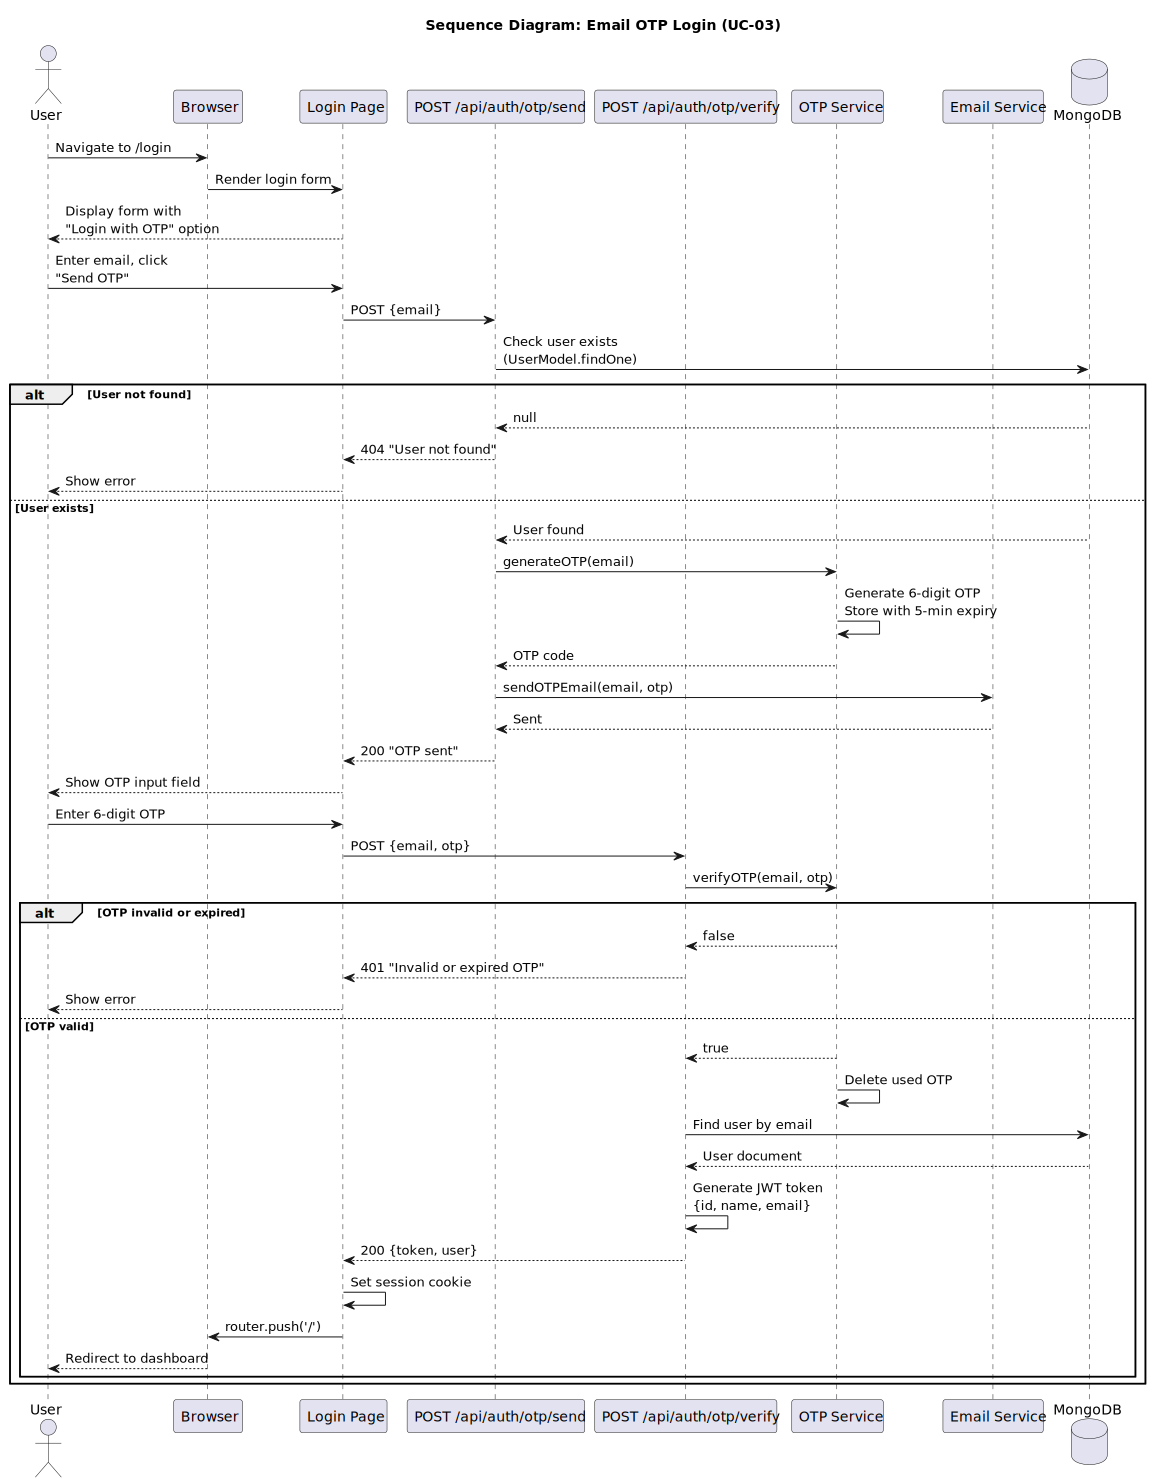
\includegraphics[width=0.9\textwidth]{diagrams/seq_otp_login.pdf}
    \caption{Sequence Diagram: Email OTP Verification (D-SQ-03)}
    \label{fig:seq_otp}
\end{figure}

\paragraph{SD-04: Create New Project}
\begin{figure}[H]
    \centering
    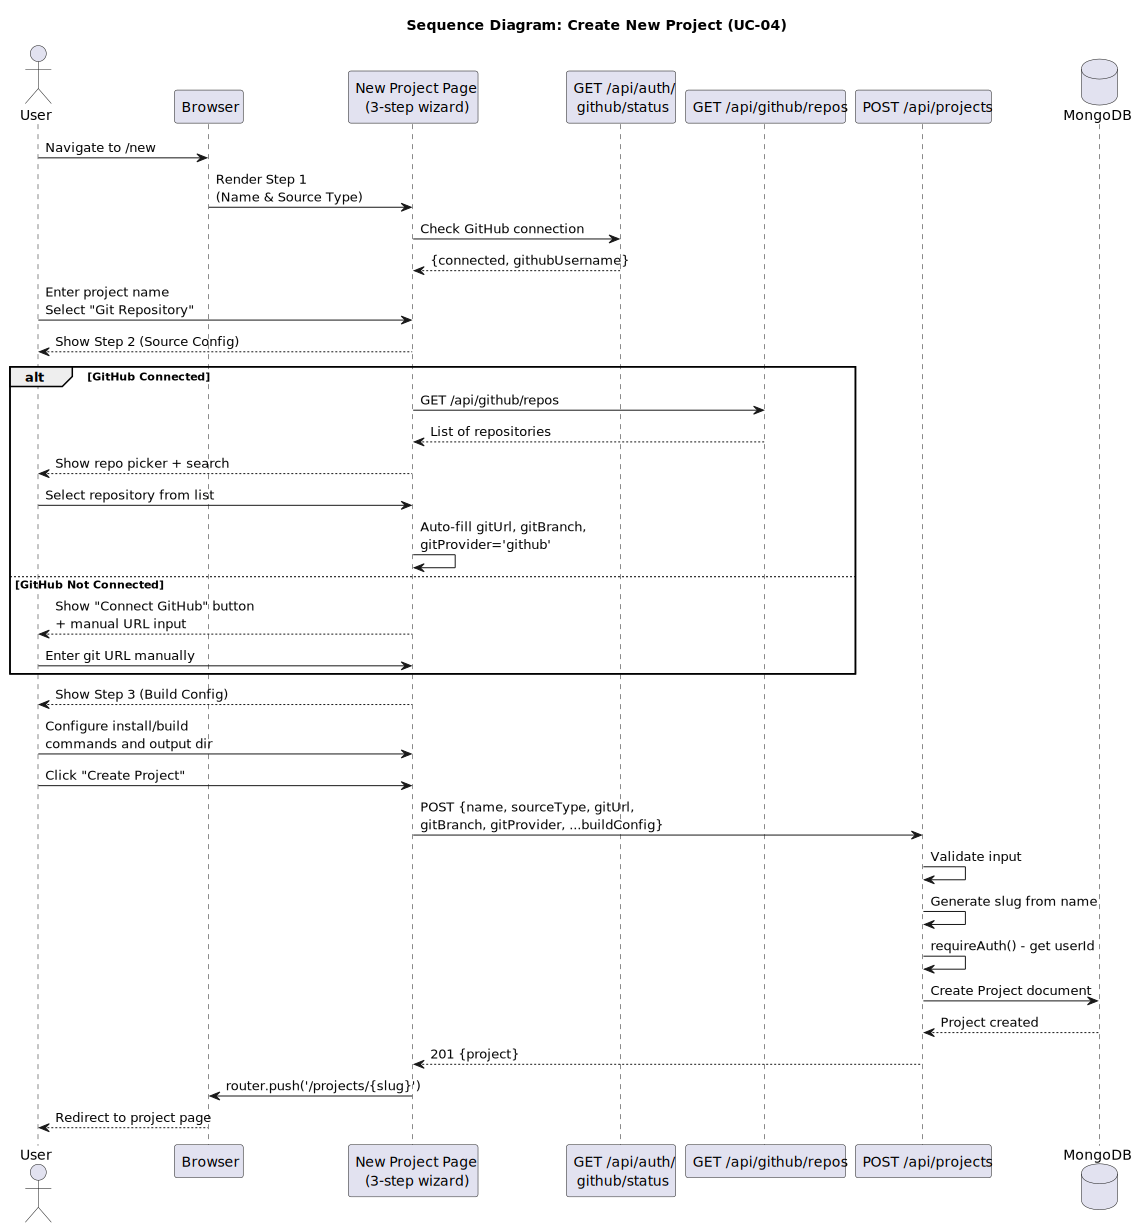
\includegraphics[width=0.95\textwidth]{diagrams/seq_create_project.pdf}
    \caption{Sequence Diagram: Create New Project (D-SQ-04)}
    \label{fig:seq_create}
\end{figure}

\paragraph{SD-05: Trigger Deployment and Build Process}
\begin{figure}[H]
    \centering
    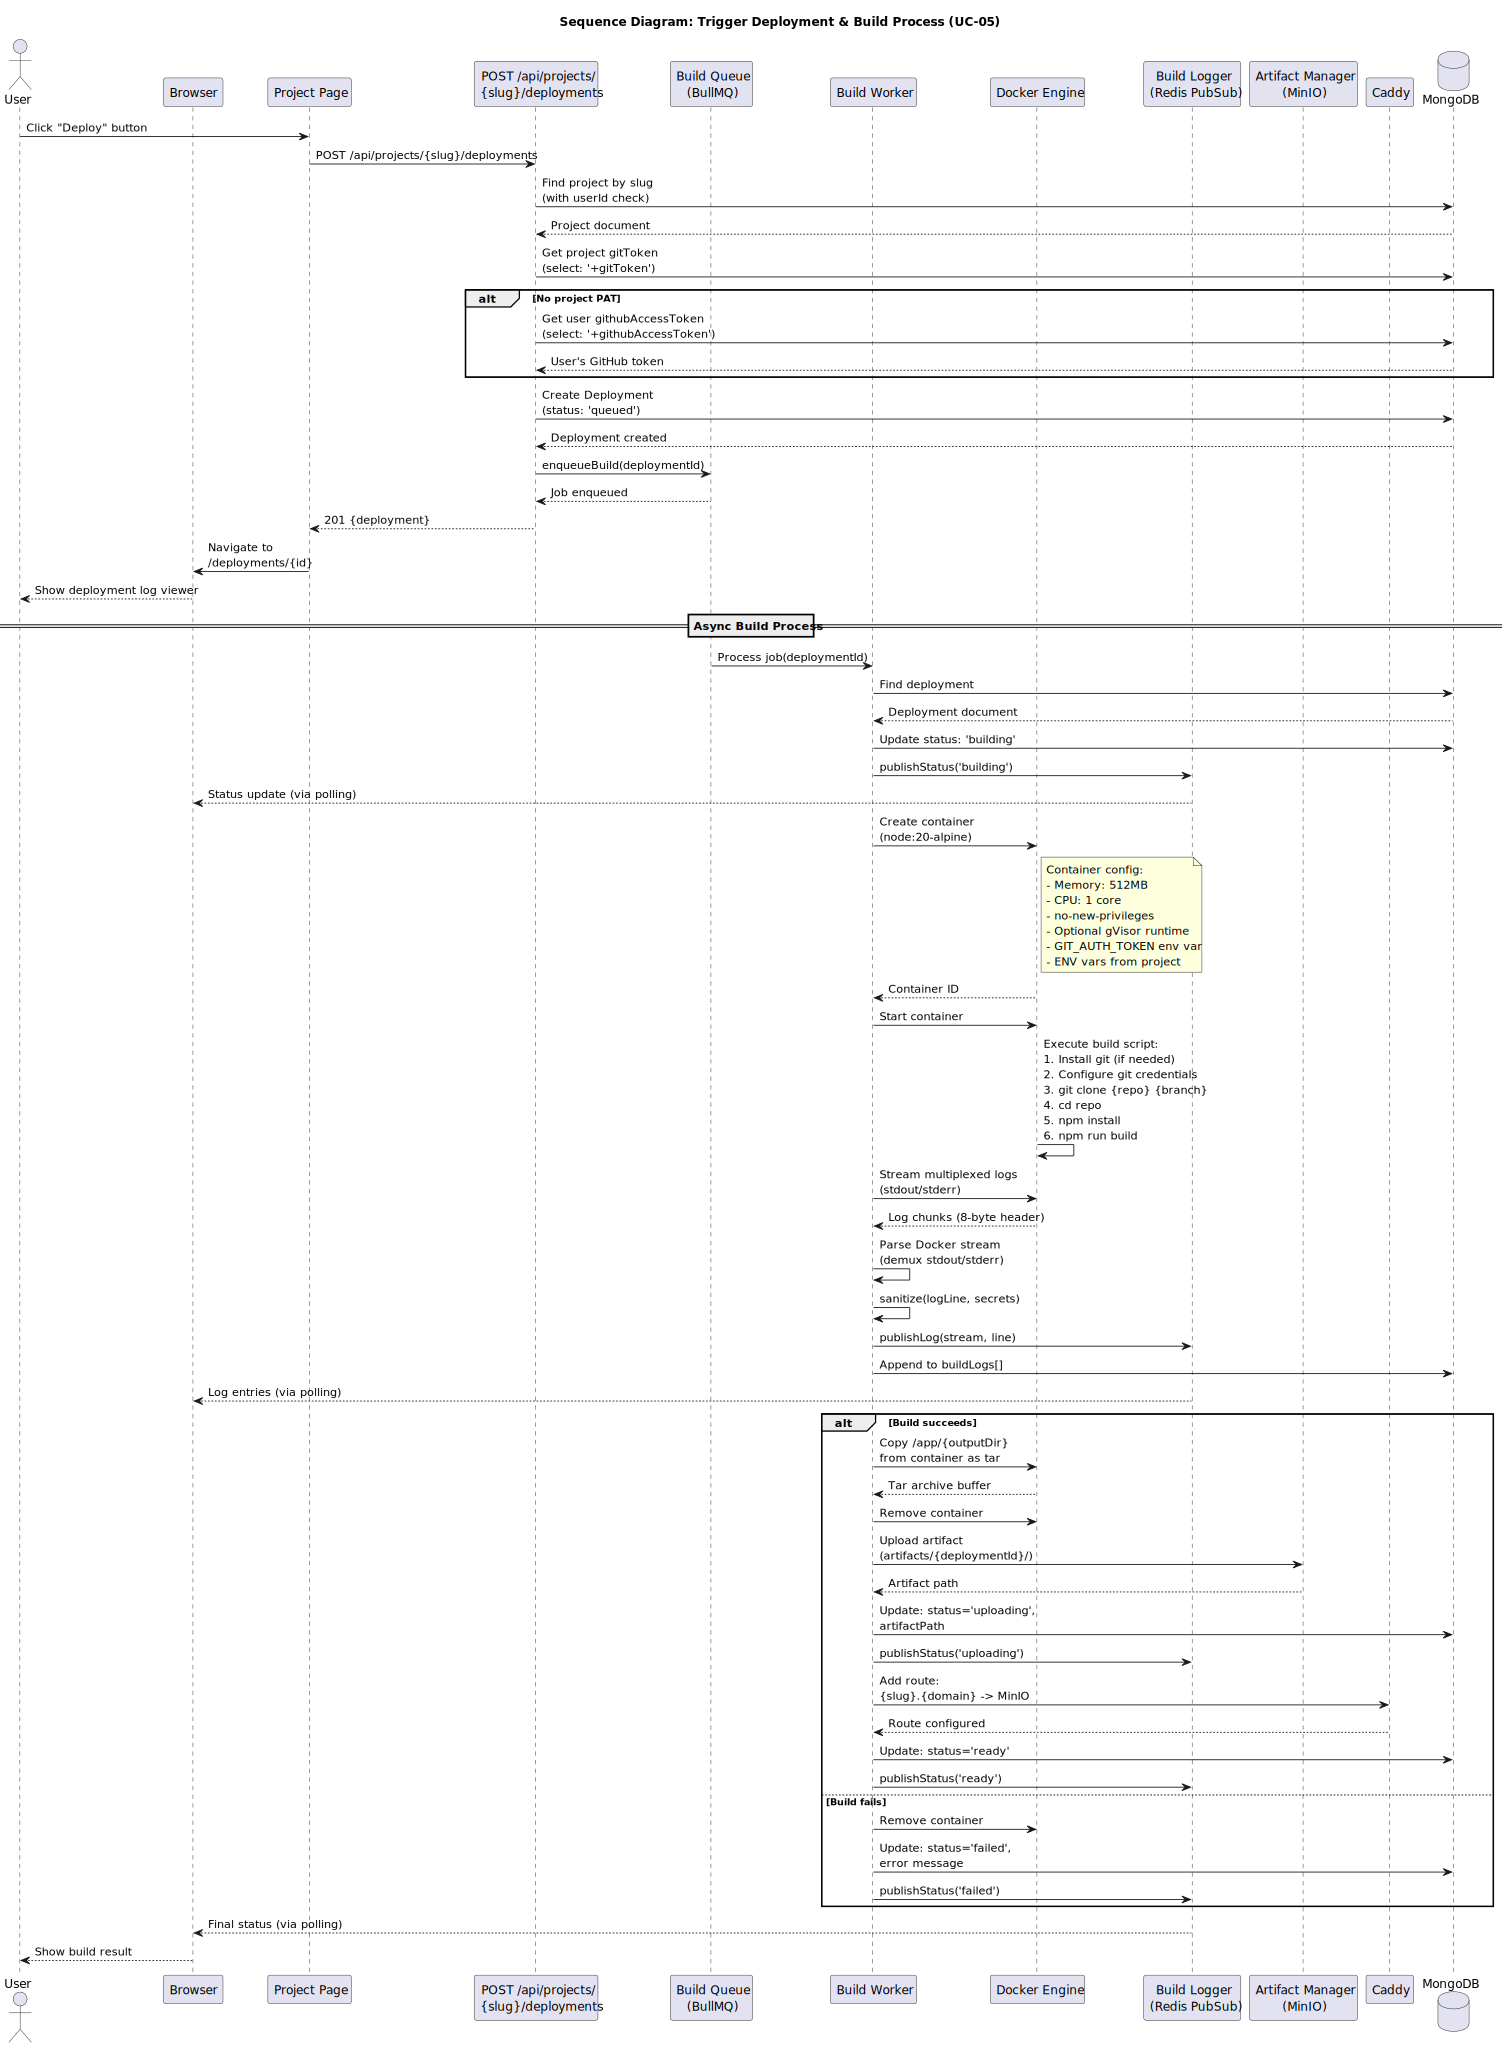
\includegraphics[width=\textwidth]{diagrams/seq_deploy.pdf}
    \caption{Sequence Diagram: Deployment and Build Process (D-SQ-05)}
    \label{fig:seq_deploy}
\end{figure}

\paragraph{SD-06: GitHub OAuth Connection}
\begin{figure}[H]
    \centering
    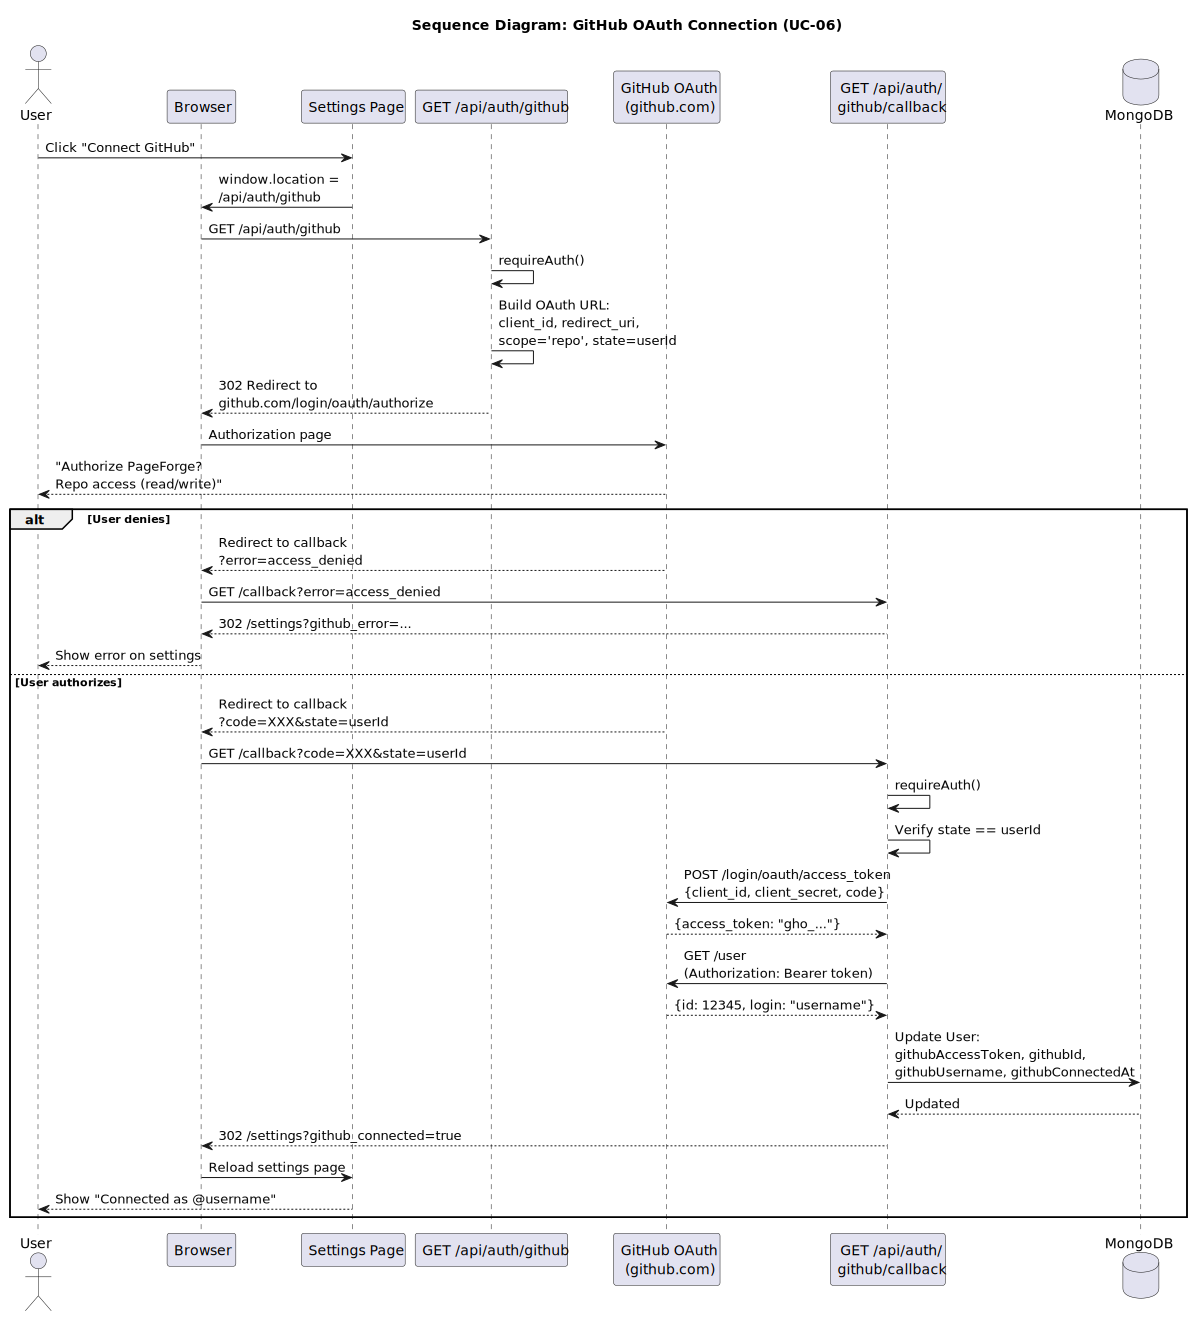
\includegraphics[width=0.9\textwidth]{diagrams/seq_github_oauth.pdf}
    \caption{Sequence Diagram: GitHub OAuth Connection (D-SQ-06)}
    \label{fig:seq_github}
\end{figure}

\paragraph{SD-07: Custom Domain Management}
\begin{figure}[H]
    \centering
    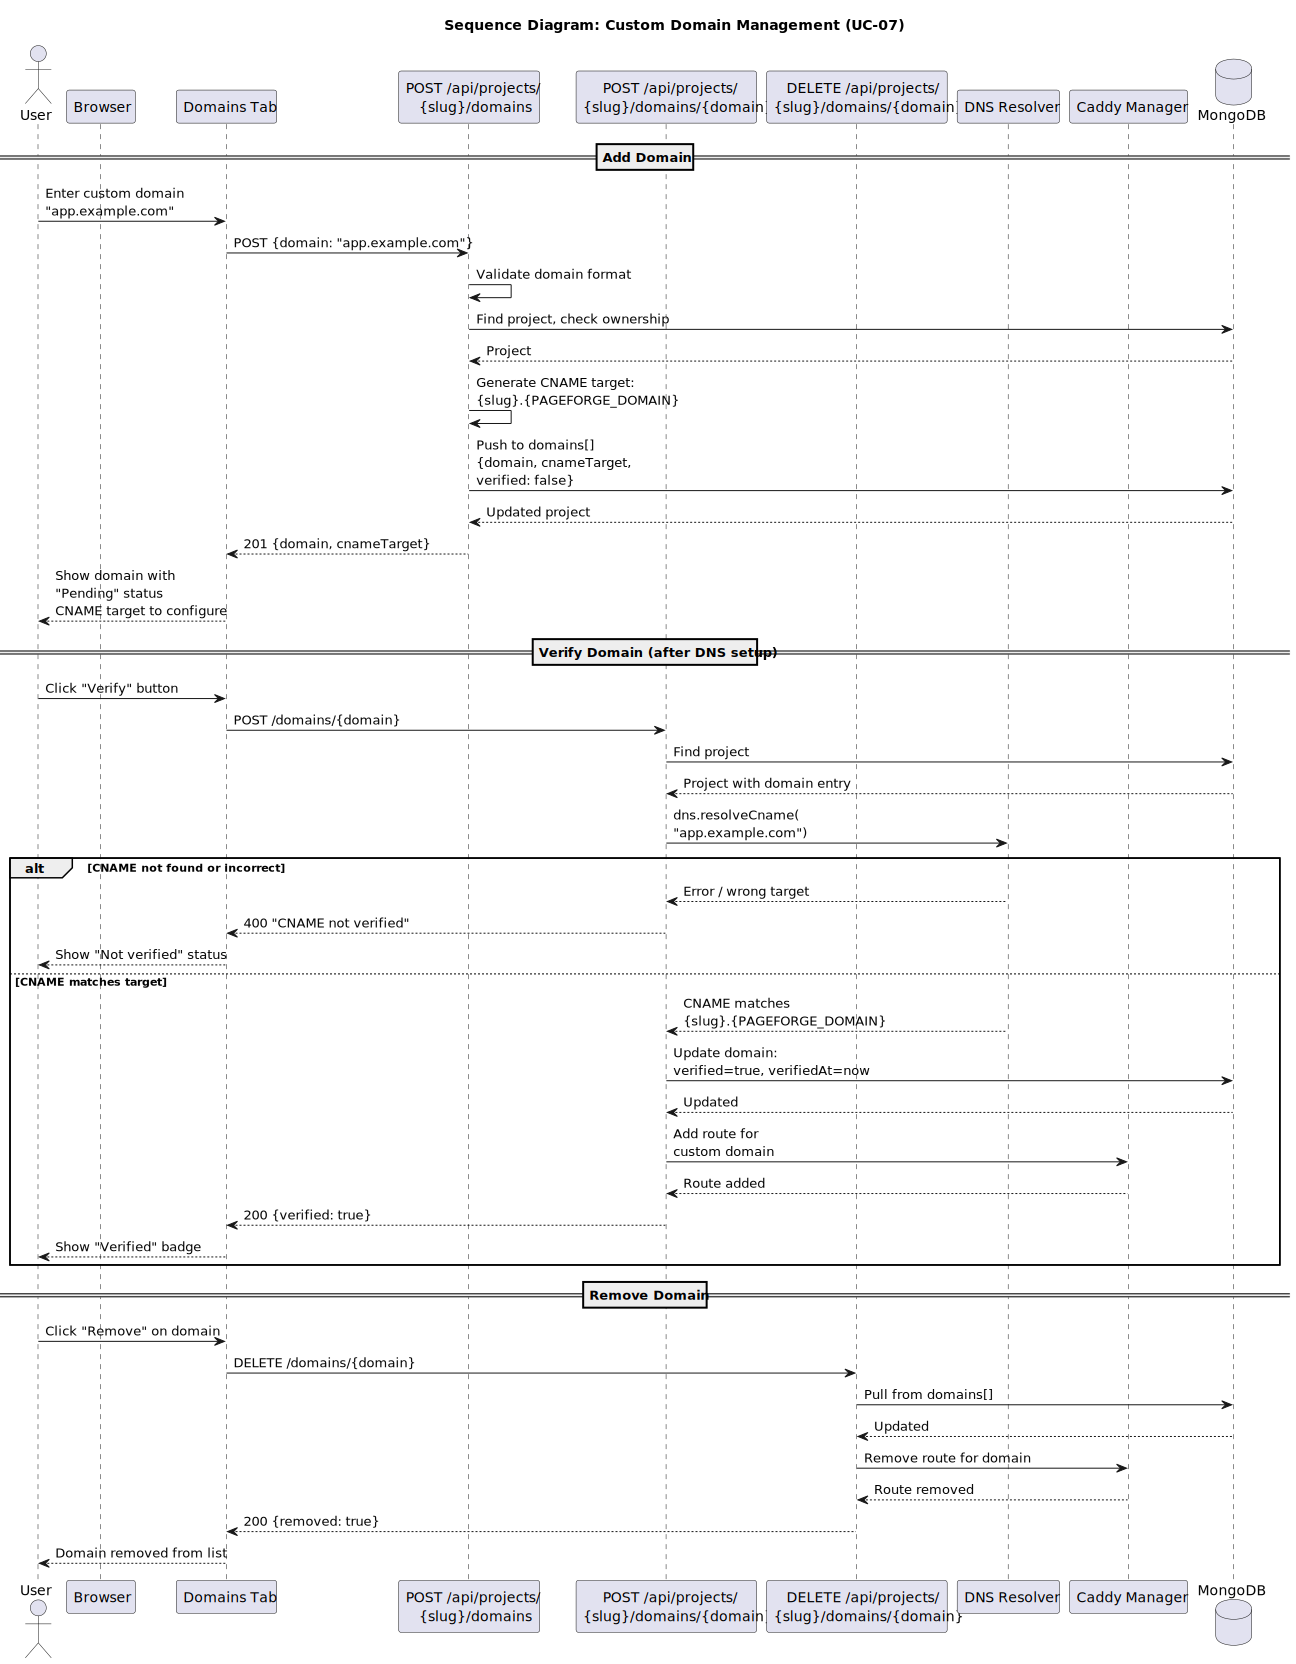
\includegraphics[width=0.95\textwidth]{diagrams/seq_domain.pdf}
    \caption{Sequence Diagram: Custom Domain Management (D-SQ-07)}
    \label{fig:seq_domain}
\end{figure}

\paragraph{SD-08: ZIP Upload and Deploy}
\begin{figure}[H]
    \centering
    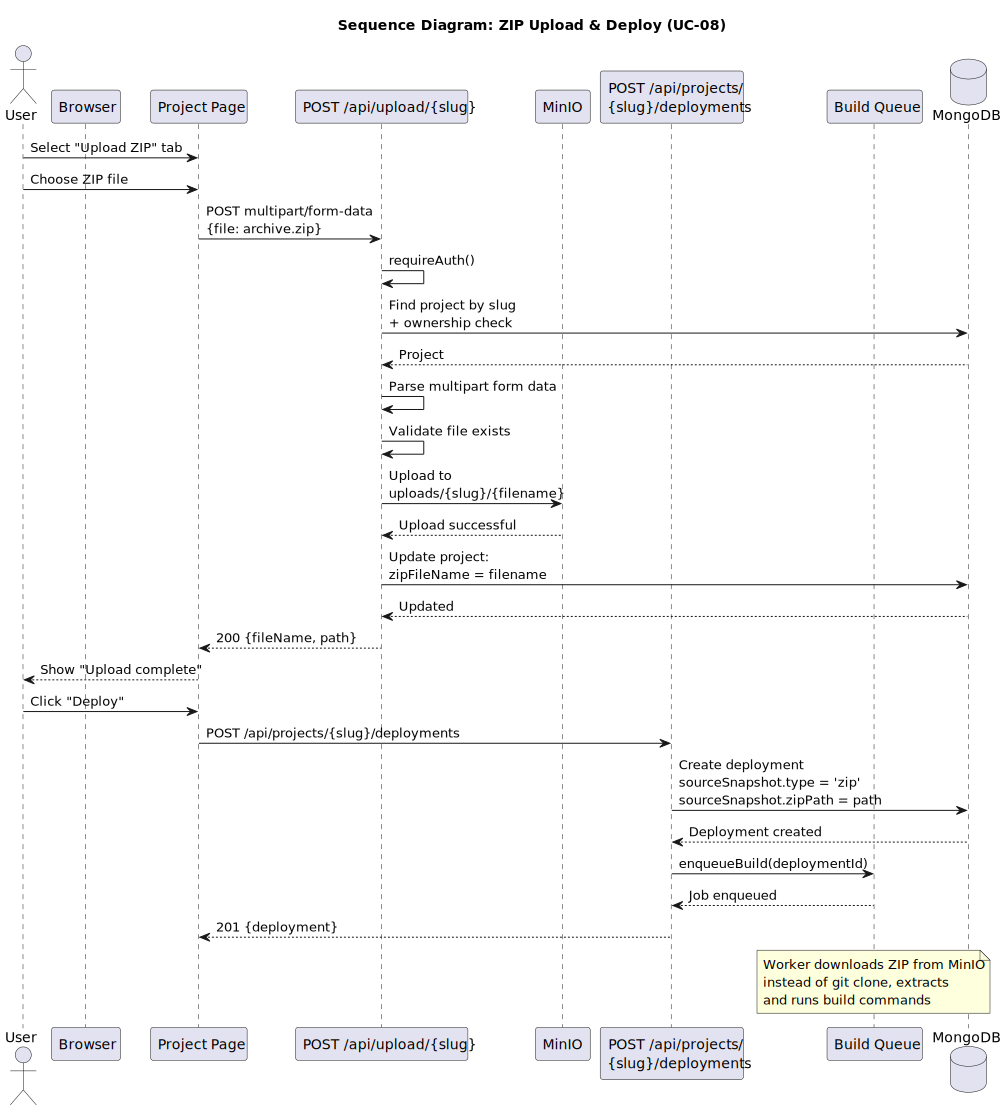
\includegraphics[width=0.9\textwidth]{diagrams/seq_upload_zip.pdf}
    \caption{Sequence Diagram: ZIP Upload and Deploy (D-SQ-08)}
    \label{fig:seq_zip}
\end{figure}

\paragraph{SD-09: Environment Variable Management}
\begin{figure}[H]
    \centering
    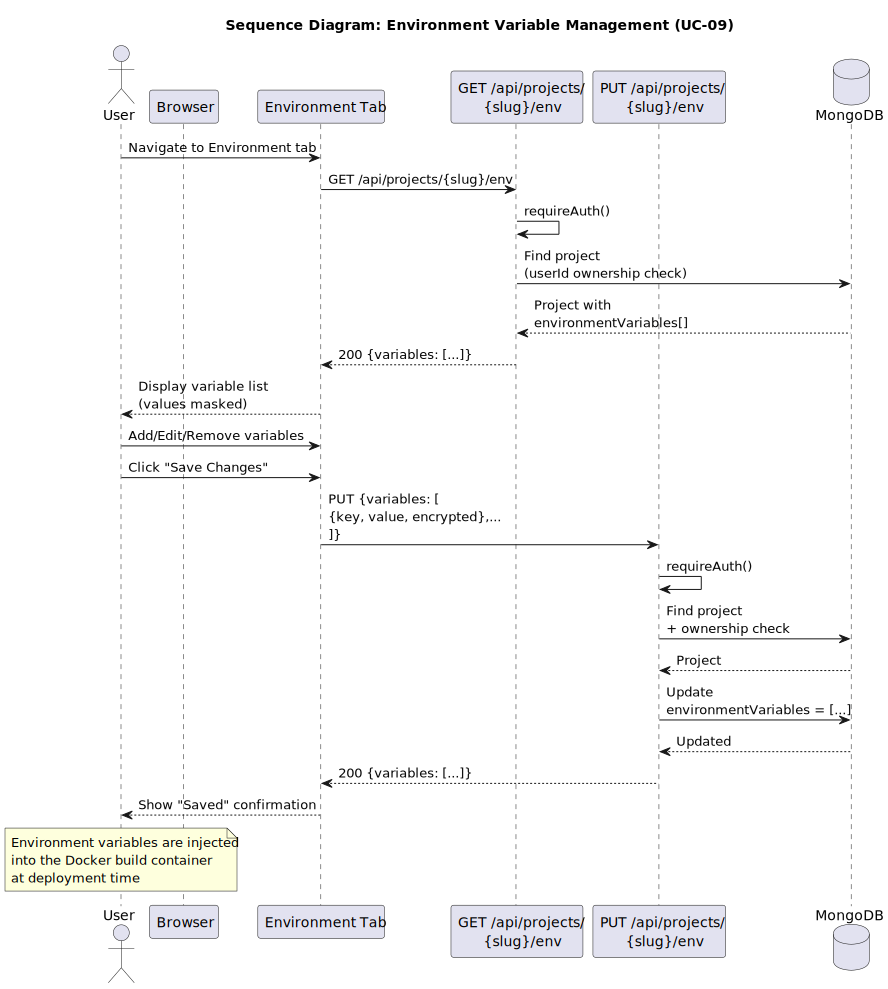
\includegraphics[width=0.85\textwidth]{diagrams/seq_env_vars.pdf}
    \caption{Sequence Diagram: Environment Variable Management (D-SQ-09)}
    \label{fig:seq_env}
\end{figure}

\paragraph{SD-10: Authentication Middleware Flow}
\begin{figure}[H]
    \centering
    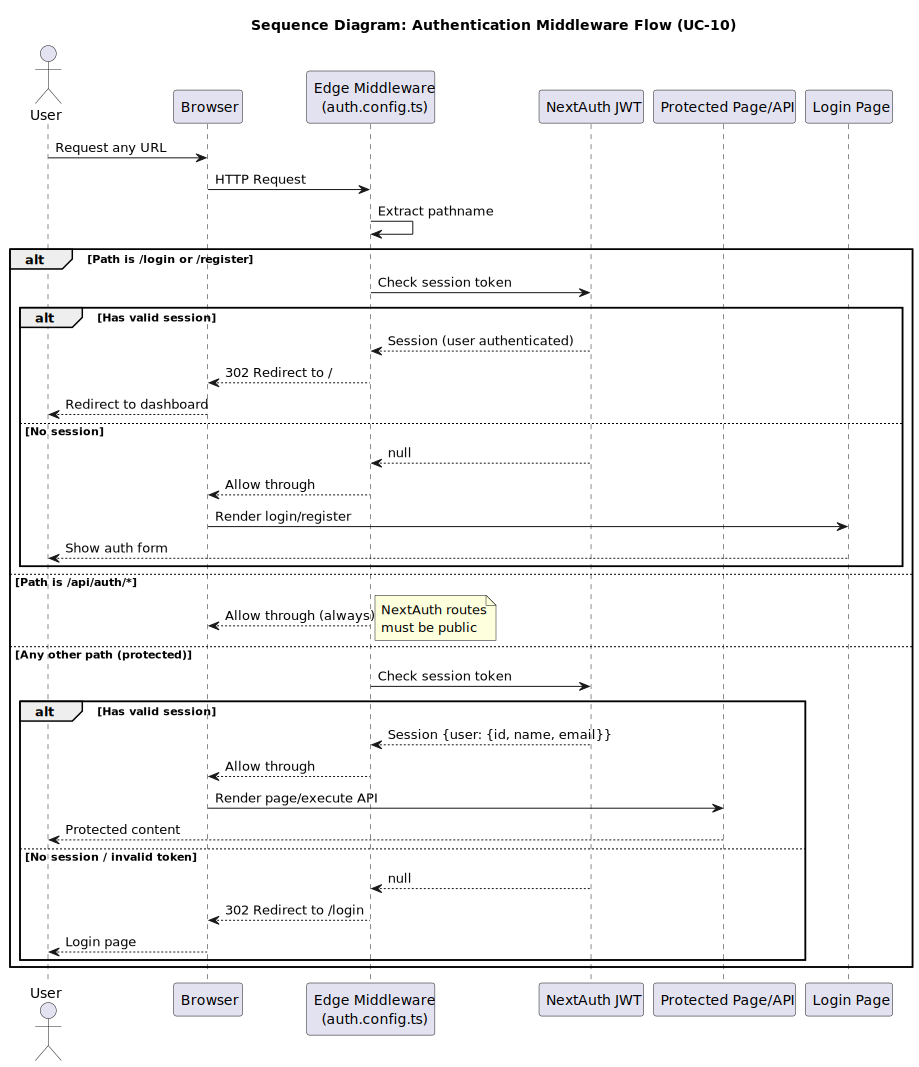
\includegraphics[width=0.85\textwidth]{diagrams/seq_middleware.pdf}
    \caption{Sequence Diagram: Authentication Middleware Flow (D-SQ-10)}
    \label{fig:seq_mw}
\end{figure}

\subsection{Database Schema}
PageForge uses MongoDB as its primary database with Mongoose as the ODM. The schema consists of three collections with embedded sub-documents.

\begin{figure}[H]
    \centering
    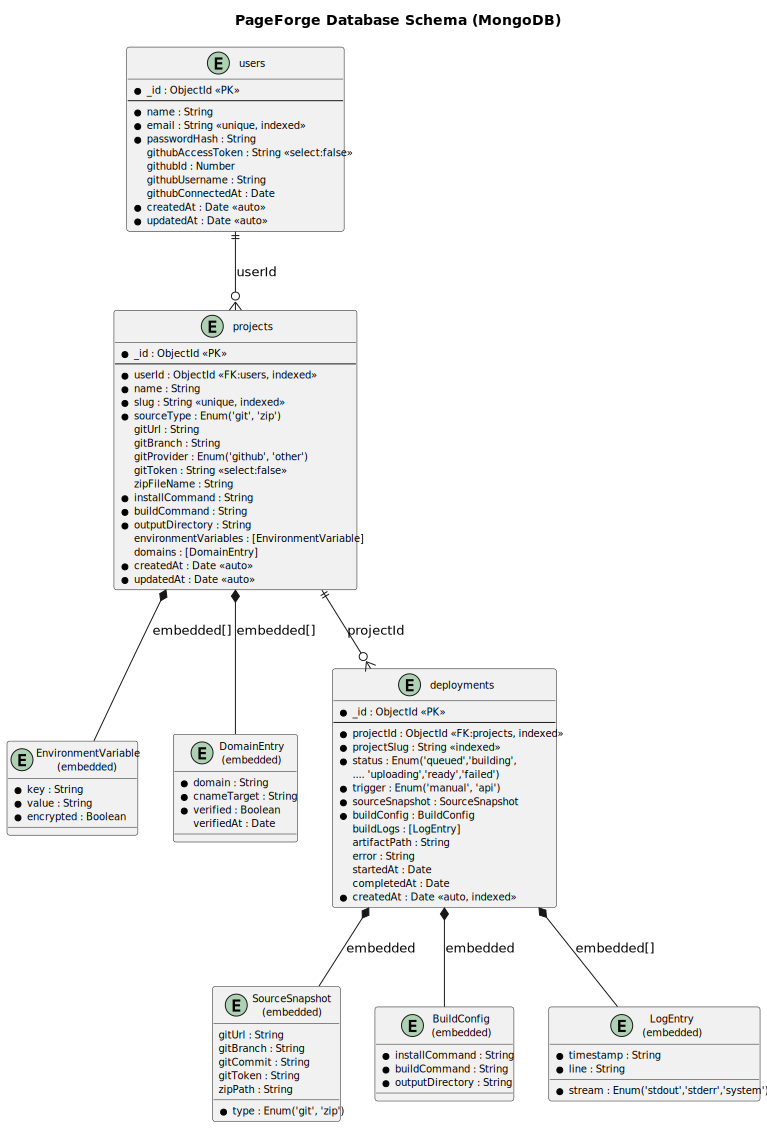
\includegraphics[width=\textwidth]{diagrams/database_schema.pdf}
    \caption{Database Entity-Relationship Diagram (D-DB-01)}
    \label{fig:db}
\end{figure}

\subsubsection{Collection: \texttt{users}}
{\small
\begin{longtable}{|l|l|l|>{\raggedright\arraybackslash}p{4.5cm}|}
\hline
\textbf{Field} & \textbf{Type} & \textbf{Constraints} & \textbf{Description} \\
\hline
\endfirsthead
\hline
\textbf{Field} & \textbf{Type} & \textbf{Constraints} & \textbf{Description} \\
\hline
\endhead
\_id & ObjectId & PK, auto & Primary key \\
\hline
name & String & required & User display name \\
\hline
email & String & required, unique, indexed & Login identifier (lowercase, trimmed) \\
\hline
passwordHash & String & required, select:false & bcrypt hash (12 rounds) \\
\hline
githubAccessToken & String & select:false & GitHub OAuth token \\
\hline
githubId & Number & & GitHub user ID \\
\hline
githubUsername & String & & GitHub login name \\
\hline
githubConnectedAt & Date & & When GitHub was connected \\
\hline
createdAt & Date & auto & Mongoose timestamp \\
\hline
updatedAt & Date & auto & Mongoose timestamp \\
\hline
\end{longtable}
}

\subsubsection{Collection: \texttt{projects}}
{\small
\begin{longtable}{|l|l|l|>{\raggedright\arraybackslash}p{4cm}|}
\hline
\textbf{Field} & \textbf{Type} & \textbf{Constraints} & \textbf{Description} \\
\hline
\endfirsthead
\hline
\textbf{Field} & \textbf{Type} & \textbf{Constraints} & \textbf{Description} \\
\hline
\endhead
\_id & ObjectId & PK, auto & Primary key \\
\hline
userId & ObjectId & required, indexed, ref:User & Owner reference \\
\hline
name & String & required & Project display name \\
\hline
slug & String & required, unique, indexed & URL-safe identifier \\
\hline
sourceType & String & required, enum:[git,zip] & Deployment source \\
\hline
gitUrl & String & & Repository URL \\
\hline
gitBranch & String & default: ``main'' & Branch to build \\
\hline
gitProvider & String & enum:[github,other] & Git hosting provider \\
\hline
gitToken & String & select:false & Per-project PAT \\
\hline
zipFileName & String & & Uploaded ZIP filename \\
\hline
installCommand & String & default: ``npm install'' & Install step \\
\hline
buildCommand & String & default: ``npm run build'' & Build step \\
\hline
outputDirectory & String & default: ``dist'' & Build output path \\
\hline
environmentVariables & Array & embedded & Build-time env vars \\
\hline
domains & Array & embedded & Custom domain entries \\
\hline
createdAt & Date & auto & Mongoose timestamp \\
\hline
updatedAt & Date & auto & Mongoose timestamp \\
\hline
\end{longtable}
}

\subsubsection{Collection: \texttt{deployments}}
{\small
\begin{longtable}{|l|l|l|>{\raggedright\arraybackslash}p{4cm}|}
\hline
\textbf{Field} & \textbf{Type} & \textbf{Constraints} & \textbf{Description} \\
\hline
\endfirsthead
\hline
\textbf{Field} & \textbf{Type} & \textbf{Constraints} & \textbf{Description} \\
\hline
\endhead
\_id & ObjectId & PK, auto & Primary key \\
\hline
projectId & ObjectId & required, indexed, ref:Project & Parent project \\
\hline
projectSlug & String & required, indexed & Denormalized slug \\
\hline
status & String & required, enum & Build lifecycle state \\
\hline
trigger & String & required, enum:[manual,api] & How deployment started \\
\hline
sourceSnapshot & Object & required, embedded & Frozen source config \\
\hline
buildConfig & Object & required, embedded & Frozen build commands \\
\hline
buildLogs & Array & embedded & Log entries array \\
\hline
artifactPath & String & & MinIO artifact location \\
\hline
error & String & & Error message on failure \\
\hline
startedAt & Date & & Build start time \\
\hline
completedAt & Date & & Build end time \\
\hline
createdAt & Date & auto, indexed & Creation timestamp \\
\hline
\end{longtable}
}

\subsubsection{Indexes}
\begin{itemize}
    \item \texttt{users.email} --- unique index for login lookup.
    \item \texttt{projects.slug} --- unique index for URL routing.
    \item \texttt{projects.userId} --- index for user-scoped queries.
    \item \texttt{deployments.projectId} --- index for project-scoped queries.
    \item \texttt{deployments.projectSlug} --- index for slug-based lookups.
    \item \texttt{deployments.createdAt} --- index for chronological sorting.
\end{itemize}

\subsection{Security Design}

\subsubsection{Authentication and Authorization Mechanisms}

\paragraph{Authentication Mechanisms (D-SEC-01)}
\begin{enumerate}
    \item \textbf{Password-Based Authentication:}
    \begin{itemize}
        \item Passwords are hashed using bcrypt with 12 salt rounds.
        \item Plaintext passwords are never stored or logged.
        \item Authentication is handled by NextAuth.js v5 Credentials provider.
        \item JWT tokens are issued with 30-day maximum age.
        \item Tokens contain user ID, name, and email (no sensitive data).
    \end{itemize}

    \item \textbf{OTP-Based Verification:}
    \begin{itemize}
        \item 6-digit cryptographically random OTP generated per request.
        \item OTPs expire after 5 minutes.
        \item Single-use: invalidated immediately after successful verification.
        \item Delivered via email to the registered address.
        \item Used for two purposes: (1) email verification during registration, (2) identity verification during password reset.
    \end{itemize}

    \item \textbf{JWT Session Management:}
    \begin{itemize}
        \item Strategy: JWT (stateless, no server-side session store).
        \item Token stored in HTTP-only secure cookie.
        \item Maximum age: 30 days.
        \item Token payload: \texttt{\{id, name, email\}}.
    \end{itemize}
\end{enumerate}

\paragraph{Authorization Mechanisms (D-SEC-02)}
\begin{enumerate}
    \item \textbf{Route Protection via Middleware:}
    \begin{itemize}
        \item All routes except \texttt{/login}, \texttt{/register}, and \texttt{/api/auth/*} require authentication.
        \item Middleware runs in Edge Runtime for performance.
        \item Unauthenticated requests are redirected to \texttt{/login}.
        \item Authenticated users are redirected away from auth pages.
    \end{itemize}

    \item \textbf{API-Level Ownership Checks:}
    \begin{itemize}
        \item All 8 protected API route files call \texttt{requireAuth()} which extracts \texttt{userId} from the JWT.
        \item All database queries include \texttt{userId} filter to enforce ownership scoping.
        \item Users can only access their own projects, deployments, and settings.
    \end{itemize}

    \item \textbf{GitHub OAuth Security:}
    \begin{itemize}
        \item OAuth state parameter contains \texttt{userId} to prevent CSRF.
        \item Callback verifies \texttt{state} matches the authenticated user's ID.
        \item Redirect URI uses \texttt{AUTH\_URL} (not request origin) to prevent open redirect.
        \item \texttt{trustHost: true} in NextAuth config for reverse proxy compatibility.
    \end{itemize}
\end{enumerate}

\subsubsection{Security Protocols}

\paragraph{SP-01: Secret Management}
\begin{itemize}
    \item \textbf{Password hashes:} Stored with Mongoose \texttt{select: false}; stripped in \texttt{toJSON}/\texttt{toObject} transforms.
    \item \textbf{GitHub access tokens:} Stored with \texttt{select: false}; never exposed in API responses; only a \texttt{hasGithubToken} boolean is returned.
    \item \textbf{Project PATs:} Stored with \texttt{select: false}; only \texttt{hasGitToken} boolean is exposed.
    \item \textbf{Auth secret:} \texttt{AUTH\_SECRET} environment variable for JWT signing; never exposed.
\end{itemize}

\paragraph{SP-02: Build Container Isolation}
\begin{itemize}
    \item Builds execute in ephemeral Docker containers destroyed after each build.
    \item Containers have \texttt{no-new-privileges} security option.
    \item Resource limits: configurable memory (default 512MB) and CPU (default 1 core).
    \item Optional gVisor (\texttt{runsc}) runtime for additional kernel-level sandboxing.
    \item Git credentials passed via environment variable (not command-line arguments) to avoid \texttt{/proc} exposure.
    \item Git credential helper configured inside the container to use the token without embedding in URLs.
\end{itemize}

\paragraph{SP-03: Log Sanitization}
\begin{itemize}
    \item The \texttt{sanitize()} function replaces all known secrets in build log output with \texttt{[REDACTED]}.
    \item Secrets sanitized include: \texttt{GIT\_AUTH\_TOKEN}, project PAT, user OAuth token, and all environment variable values.
    \item Sanitization is applied before both Redis publishing and MongoDB persistence.
\end{itemize}

\paragraph{SP-04: Reverse Proxy Security}
\begin{itemize}
    \item Caddy handles TLS termination and HTTPS enforcement.
    \item \texttt{trustHost: true} in NextAuth config trusts \texttt{X-Forwarded-*} headers from the proxy.
    \item \texttt{AUTH\_URL} is used as the canonical base URL for all redirect construction (prevents localhost leakage behind proxies).
    \item Cloudflare Tunnel (optional) provides DDoS protection and hides origin server IP.
\end{itemize}

\paragraph{SP-05: Data Access Control}
\begin{itemize}
    \item All API routes extract \texttt{userId} from the JWT and filter database queries accordingly.
    \item No cross-user data access is possible through the API.
    \item Deployment artifacts are stored in MinIO with deployment-specific paths.
    \item Caddy routes are configured per-project to serve only the correct artifacts.
\end{itemize}

\newpage

%===============================================================
% SECTION 5: OTHER NONFUNCTIONAL REQUIREMENTS
%===============================================================
\section{Other Nonfunctional Requirements}

\subsection{Performance Requirements}
\begin{description}
    \item[NFR-01] Dashboard pages shall load within 2 seconds on a standard broadband connection.
    \item[NFR-02] API responses for CRUD operations shall complete within 500ms.
    \item[NFR-03] Build log streaming latency shall be under 1 second from worker to browser.
    \item[NFR-04] The system shall handle concurrent builds limited by Docker resource availability.
    \item[NFR-05] Deployment status polling interval shall be 2 seconds.
    \item[NFR-06] GitHub repository listing shall support pagination (configurable \texttt{per\_page}, default 30).
\end{description}

\subsection{Safety Requirements}
\begin{description}
    \item[NFR-07] Build containers shall be resource-limited to prevent denial-of-service to the host system.
    \item[NFR-08] Failed builds shall not leave orphaned Docker containers (cleanup on both success and failure).
    \item[NFR-09] Build failures shall not affect other running builds or the main application.
\end{description}

\subsection{Security Requirements}
\begin{description}
    \item[NFR-10] All passwords shall be hashed with bcrypt (minimum 12 rounds).
    \item[NFR-11] Sensitive fields shall use Mongoose \texttt{select: false} and be stripped from API responses.
    \item[NFR-12] Build containers shall run with \texttt{no-new-privileges} security option.
    \item[NFR-13] All secrets shall be sanitized from build logs before storage and streaming.
    \item[NFR-14] JWT tokens shall expire after a maximum of 30 days.
    \item[NFR-15] API routes shall enforce ownership checks (users can only access their own data).
    \item[NFR-16] GitHub OAuth shall use the \texttt{state} parameter to prevent CSRF attacks.
\end{description}

\subsection{Software Quality Attributes}
\begin{description}
    \item[NFR-17] \textbf{Maintainability:} Monorepo with shared types ensures consistency across web app and worker.
    \item[NFR-18] \textbf{Portability:} Runs on any Linux server with Docker; no cloud-provider-specific dependencies.
    \item[NFR-19] \textbf{Usability:} Dark mode default, responsive design, loading/error/empty states on all pages.
    \item[NFR-20] \textbf{Reliability:} BullMQ provides job retry and persistence; deployments survive worker restarts.
    \item[NFR-21] \textbf{Extensibility:} Git provider type supports ``other'' for future self-hosted Git integration.
\end{description}

\subsection{Business Rules}
\begin{description}
    \item[BR-01] Open registration: any user can create an account.
    \item[BR-02] Projects are scoped per user: users can only see and manage their own projects.
    \item[BR-03] Token priority for private repos: project-level PAT takes precedence over user-level GitHub OAuth token.
    \item[BR-04] Only the latest successful deployment is actively served via Caddy (previous deployments remain in storage).
    \item[BR-05] Custom domains require DNS CNAME verification before activation.
\end{description}

\newpage

%===============================================================
% SECTION 6: TRACEABILITY
%===============================================================
\section{Traceability}

\subsection{Requirement-to-Design Mapping}

{\footnotesize
\begin{longtable}{|>{\raggedright\arraybackslash}p{2.2cm}|>{\raggedright\arraybackslash}p{2.5cm}|>{\raggedright\arraybackslash}p{3cm}|>{\raggedright\arraybackslash}p{4cm}|}
\hline
\textbf{Req / UC ID} & \textbf{Req / UC Name} & \textbf{Design ID(s)} & \textbf{Design Artifact} \\
\hline
\endfirsthead
\hline
\textbf{Req / UC ID} & \textbf{Req / UC Name} & \textbf{Design ID(s)} & \textbf{Design Artifact} \\
\hline
\endhead

UC-01 & User Registration & D-CL-01, D-SQ-01, D-DB-01 & Class Diagram, Sequence Diagram, Database Schema \\
\hline
UC-02 & User Login (Credentials) & D-CL-01, D-SQ-02, D-SEC-01 & Class Diagram, Sequence Diagram, Security Design \\
\hline
UC-03 & Email OTP Verification & D-CL-01, D-SQ-03, D-SEC-01 & Class Diagram, Sequence Diagram, Security Design \\
\hline
UC-04 & GitHub OAuth Connection & D-CL-01, D-SQ-06, D-DB-01, D-SEC-02 & Class Diagram, Sequence Diagram, Database Schema, Security Design \\
\hline
UC-05 & Project Management & D-CL-01, D-SQ-04, D-DB-01 & Class Diagram, Sequence Diagram, Database Schema \\
\hline
UC-06 & Deployment Pipeline & D-CL-01, D-SQ-05, D-DB-01, D-SEC-02 & Class Diagram, Sequence Diagram, Database Schema, Security Design \\
\hline
UC-07 & Environment Variables & D-CL-01, D-SQ-09, D-DB-01 & Class Diagram, Sequence Diagram, Database Schema \\
\hline
UC-08 & Custom Domain Mgmt & D-CL-01, D-SQ-07, D-DB-01 & Class Diagram, Sequence Diagram, Database Schema \\
\hline
UC-09 & ZIP File Upload & D-CL-01, D-SQ-08, D-DB-01 & Class Diagram, Sequence Diagram, Database Schema \\
\hline
UC-10 & Build Log Viewer & D-CL-01, D-SQ-05, D-SQ-10 & Class Diagram, Sequence Diagrams \\
\hline
UC-11 & Forgot Password & D-CL-01, D-SQ-03, D-SEC-01 & Class Diagram, Sequence Diagram, Security Design \\
\hline
FR-01 to FR-07 & Registration Reqs & D-SQ-01, D-DB-01 & Sequence Diagram, Database Schema \\
\hline
FR-08 to FR-14 & Login (Credentials) & D-SQ-02, D-SEC-01 & Sequence Diagram, Security Design \\
\hline
FR-15 to FR-22 & Email OTP Verification Reqs & D-SQ-03, D-SEC-01 & Sequence Diagram, Security Design \\
\hline
FR-23 to FR-30 & GitHub OAuth Reqs & D-SQ-06, D-SEC-02 & Sequence Diagram, Security Design \\
\hline
FR-31 to FR-43 & Project Mgmt Reqs & D-SQ-04, D-DB-01 & Sequence Diagram, Database Schema \\
\hline
FR-44 to FR-65 & Deployment Reqs & D-SQ-05, D-DB-01, D-SEC-02 & Sequence Diagram, Database Schema, Security Design \\
\hline
FR-66 to FR-70 & Env Variables Reqs & D-SQ-09, D-DB-01 & Sequence Diagram, Database Schema \\
\hline
FR-71 to FR-77 & Domain Mgmt Reqs & D-SQ-07, D-DB-01 & Sequence Diagram, Database Schema \\
\hline
FR-78 to FR-81 & ZIP Upload Reqs & D-SQ-08, D-DB-01 & Sequence Diagram, Database Schema \\
\hline
FR-82 to FR-88 & Log Viewer Reqs & D-SQ-05, D-SQ-10 & Sequence Diagrams \\
\hline
FR-89 to FR-98 & Forgot Password Reqs & D-SQ-03, D-SEC-01 & Sequence Diagram, Security Design \\
\hline
NFR-10 & Password Hashing & D-SEC-01 & Security Design \\
\hline
NFR-11 & Sensitive Field Protection & D-SEC-01, D-DB-01 & Security Design, Database Schema \\
\hline
NFR-12 & Container Security & D-SEC-02 & Security Design \\
\hline
NFR-13 & Log Sanitization & D-SEC-02 & Security Design \\
\hline
NFR-14 & JWT Expiry & D-SEC-01 & Security Design \\
\hline
NFR-15 & Ownership Checks & D-SEC-02, D-SQ-10 & Security Design, Sequence Diagram \\
\hline
NFR-16 & OAuth CSRF Prevention & D-SEC-02 & Security Design \\
\hline
\end{longtable}
}

% Reset heading definitions to defaults (remove \needspace that causes excessive page breaks)
\makeatletter
\renewcommand\section{\@startsection{section}{1}{\z@}%
  {-3.5ex \@plus -1ex \@minus -.2ex}%
  {2.3ex \@plus .2ex}%
  {\normalfont\Large\bfseries}}
\renewcommand\subsection{\@startsection{subsection}{2}{\z@}%
  {-3.25ex\@plus -1ex \@minus -.2ex}%
  {1.5ex \@plus .2ex}%
  {\normalfont\large\bfseries}}
\renewcommand\subsubsection{\@startsection{subsubsection}{3}{\z@}%
  {-3.25ex\@plus -1ex \@minus -.2ex}%
  {1.5ex \@plus .2ex}%
  {\normalfont\normalsize\bfseries}}
\renewcommand\paragraph{\@startsection{paragraph}{4}{\z@}%
  {3.25ex \@plus 1ex \@minus .2ex}%
  {-1em}%
  {\normalfont\normalsize\bfseries}}
\makeatother

\newpage

%===============================================================
% SECTION 7: OTHER REQUIREMENTS
%===============================================================
\section{Other Requirements}
\begin{itemize}
    \item \textbf{Database:} MongoDB 7.0+ with Mongoose ODM. Connection pooling with cached connection pattern.
    \item \textbf{Internationalization:} Not in scope for v1.0. English only.
    \item \textbf{Legal:} Self-hosted; no data leaves the user's infrastructure (except GitHub API calls). Users are responsible for compliance with their own policies.
    \item \textbf{Reuse:} The \texttt{packages/shared} module is designed for reuse across web app and worker processes.
    \item \textbf{Deployment:} Infrastructure services are containerized via \texttt{docker-compose.yml}. Application processes (web, worker) run natively on the host.
\end{itemize}

\newpage

%===============================================================
% APPENDICES
%===============================================================
\appendix

\section{Glossary}
\begin{description}
    \item[BullMQ] A Node.js library for Redis-based message queues with job scheduling and retry support.
    \item[Caddy] A modern web server with automatic HTTPS and a JSON-based admin API for dynamic configuration.
    \item[CNAME] A DNS record type that maps one domain name to another (Canonical Name).
    \item[CSRF] Cross-Site Request Forgery --- an attack where unauthorized commands are transmitted from a trusted user.
    \item[Docker] A platform for building, shipping, and running applications in isolated containers.
    \item[gVisor] A container sandbox runtime by Google that provides additional kernel-level isolation.
    \item[JWT] JSON Web Token --- a compact, URL-safe means of representing claims to be transferred between two parties.
    \item[MinIO] An S3-compatible object storage server designed for high-performance workloads.
    \item[Mongoose] An Object Data Modeling (ODM) library for MongoDB in Node.js.
    \item[NextAuth.js] An authentication library for Next.js applications (v5 also known as Auth.js).
    \item[OAuth] An open standard for access delegation, commonly used to grant websites access to user information without exposing passwords.
    \item[OTP] One-Time Password --- a password valid for only one login session or transaction.
    \item[PAT] Personal Access Token --- a token used as an alternative to passwords for Git authentication.
    \item[Pub/Sub] Publish/Subscribe messaging pattern where senders publish messages to channels without knowledge of subscribers.
    \item[REST] Representational State Transfer --- an architectural style for designing networked applications.
    \item[SPA] Single-Page Application --- a web application that interacts with the user by dynamically rewriting the current page.
    \item[WebSocket] A communication protocol providing full-duplex communication channels over a single TCP connection.
\end{description}

\end{document}
